\documentclass[conference]{IEEEtran} \IEEEoverridecommandlockouts % ================= PACOTES =================
\usepackage[utf8]{inputenc}
\usepackage[T1]{fontenc}
\usepackage[brazil]{babel}
\usepackage{cite}
\usepackage{amsmath,amssymb,amsfonts}
\usepackage{graphicx}
\usepackage{textcomp}
\usepackage{xcolor}
\usepackage{booktabs}
\usepackage{makecell}

\usepackage{array}
\usepackage{tabularx}
\usepackage{makecell}
\usepackage{adjustbox}



\renewcommand{\arraystretch}{1.4}
\newcolumntype{Y}{>{\centering\arraybackslash}X}

\title{Moderação Participativa Assistida por IA Generativa: um Experimento de
Simulação com Agentes LLM sobre a Mitigação de Debates Improdutivos}

\author{\IEEEauthorblockN{Guilherme Moura}
\IEEEauthorblockA{\textit{Programa de Engenharia de Sistemas} \\
      \textit{e Computação(PESC/COPPE)} \\
      \textit{Universidade Federal do Rio de Janeiro} \\
      Rio de Janeiro, Brazil \\
      gpcmoura@cos.ufrj.br}
\and
\IEEEauthorblockN{Luiz Filipe Brandi}
\IEEEauthorblockA{\textit{Programa de Engenharia de Sistemas} \\
      \textit{e Computação(PESC/COPPE)} \\
      \textit{Universidade Federal do Rio de Janeiro} \\
      Rio de Janeiro, Brazil \\
      brandi@cos.ufrj.br}
\and
\IEEEauthorblockN{Ramon Chaves}
\IEEEauthorblockA{\textit{Programa de Engenharia de Sistemas} \\
      \textit{e Computação(PESC/COPPE)} \\
      \textit{Universidade Federal do Rio de Janeiro} \\
      Rio de Janeiro, Brazil \\
      ramonchaves@cos.ufrj.br}
\and
\IEEEauthorblockN{Daniel Schneider}
\IEEEauthorblockA{\textit{Programa de Engenharia de Sistemas} \\
      \textit{e Computação(PESC/COPPE)} \\
      \textit{Universidade Federal do Rio de Janeiro} \\
      Rio de Janeiro, Brazil \\
      schneider@cos.ufrj.br}
}


\begin{document}

\maketitle

\begin{abstract}
Trabalhos anteriores propuseram um modelo conceitual de cinco dimensões para a
mitigação de debates improdutivos em plataformas digitais, no qual a Moderação
Participativa (D5) atua sobre a conduta antes da publicação da mensagem. O
modelo, contudo, permanecia sem verificação empírica. Este trabalho testa
prospectivamente a dimensão D5 por meio de um experimento de simulação com
agentes baseados em \textit{Large Language Models}. Vinte personas sintéticas
polarizadas, derivadas de um dataset estruturado de um milhão de personas e
classificadas por uma regra auditável de posicionamento político, debatem em
pares sobre dois temas controversos ao longo de oito turnos, em duas condições:
sem moderação e com um moderador D5 que avalia cada mensagem candidata numa
escala ordinal de hostilidade de cinco níveis e a reformula quando o limiar é
atingido. Um juiz cego pontua cada mensagem publicada três vezes. Em um desenho
balanceado de dez células e vinte debates, a moderação reduziu a hostilidade
média de 3,15 para 1,96 na escala de 0 a 4, com efeito na mesma direção em
todas as células; a verificação de robustez sobre o corpus completo de
quarenta e dois debates confirma a magnitude. A análise por turno revela que a
moderação não impede a escalada da hostilidade, mas a retarda: sob tratamento,
o oitavo turno alcança o patamar que a condição de controle atingiu no
terceiro. Os resultados constituem uma estimativa de limite superior, obtida
sob \textit{compliance} total, e são discutidos à luz das limitações de
validação humana dos instrumentos.
\end{abstract}

\begin{IEEEkeywords}
debates improdutivos, moderação participativa, agentes LLM, incivilidade
online, personas sintéticas, simulação
\end{IEEEkeywords}

\section{Introdução}

A qualidade do debate público digital é comprometida por dinâmicas que não
decorrem de ignorância ou má-fé dos participantes, mas da própria arquitetura
sociotécnica das plataformas. Algoritmos orientados ao engajamento métrico
premiam a reação impulsiva sobre a elaboração argumentativa, e os mecanismos
de moderação disponíveis operam predominantemente de forma retrospectiva —
removendo, sinalizando ou penalizando conteúdo \textit{após} a publicação,
quando o dano à interação já se consumou. Trabalhos anteriores caracterizaram
esse fenômeno como \textit{debate improdutivo} e propuseram um modelo
conceitual de mitigação organizado em cinco dimensões, atravessadas por uma
camada transversal de mediação por Inteligência Artificial Generativa sob o
princípio da simbiose humano-IA~\cite{moura2026hostility}.

Entre essas dimensões, a Moderação Participativa (D5) ocupa uma posição
singular. Enquanto as demais qualificam o conteúdo ou estruturam a
argumentação, D5 regula a \textit{conduta}, e o faz em dois modos: proativo,
configurando o espaço discursivo antes da instauração do conflito, e reativo,
contendo a escalada durante um debate que se deteriora. É a única dimensão que
opera \textit{antes da publicação} da mensagem — no intervalo entre a redação e
a postagem —, e essa característica é justamente o que a torna difícil de
avaliar em ambientes reais: observar o efeito de uma reformulação exigiria
acesso à mensagem que não foi publicada. Em uma plataforma real, a mensagem
candidata rejeitada ou reescrita pelo autor simplesmente não existe como dado
observável, e o contrafactual — o que teria acontecido se ela tivesse sido
publicada — é inacessível por construção.

Esta restrição motiva a escolha metodológica deste trabalho. A simulação com
agentes baseados em \textit{Large Language Models} (LLMs) permite observar
simultaneamente a mensagem candidata e a mensagem publicada, tornando
mensurável aquilo que a observação naturalística não alcança. Ao instanciar
debatedores artificiais polarizados, registrar cada mensagem antes e depois da
intervenção e submeter ambas as condições a um avaliador cego, torna-se
possível estimar o efeito da moderação prospectiva sob condições controladas.
O experimento aqui descrito provoca de forma controlada as patologias do debate
improdutivo identificadas por Angenot~\cite{angenot2008dialogues} e verifica se
a intervenção prevista por D5 as mitiga.

A contribuição do trabalho é tripla. Em primeiro lugar, oferece a primeira
verificação empírica de uma das dimensões do modelo predecessor, que até então
permanecia no plano conceitual. Em segundo, propõe e documenta uma escala
ordinal de hostilidade ancorada na literatura de incivilidade política e
aplicável por instrução a agentes LLM, com fundamentação nível a nível. Em
terceiro, disponibiliza um protocolo experimental integralmente auditável, em
que cada decisão de moderação, cada pontuação e cada exclusão do corpus ficam
registradas e reanalisáveis sob critérios distintos dos aqui adotados.

\subsection{Questões de Pesquisa}

O trabalho orienta-se por três questões:

\begin{itemize}
  \item \textbf{QP1.} A moderação participativa prospectiva reduz a
        hostilidade observável em um debate polarizado entre agentes
        artificiais?
  \item \textbf{QP2.} Qual é o padrão temporal desse efeito ao longo dos
        turnos de um debate?
  \item \textbf{QP3.} Em que medida a reformulação preserva a posição
        substantiva do autor, evitando que a mitigação da hostilidade se
        converta em supressão do dissenso?
\end{itemize}

O recorte precisa ser declarado desde já: o experimento testa se o
\textit{mecanismo} funciona sobre debatedores simulados, e não como usuários
humanos reagiriam à mediação. São duas perguntas distintas, e apenas a primeira
está ao alcance deste desenho. A segunda — se autores reais aceitariam a
reformulação proposta — é investigada empiricamente por outra linha de
trabalhos~\cite{argyle2023leveraging,katsaros2022reconsidering}, e sua ausência
aqui é o que faz dos resultados uma estimativa de limite superior. A distinção
é retomada nas Seções VII e VIII.

Cabe ainda uma observação sobre o objeto medido. A hostilidade avaliada neste
trabalho é a que se manifesta no texto publicado, tal como classificada por um
agente instruído com uma rubrica explícita. Não se trata de hostilidade
percebida por leitores humanos, nem de intenção hostil do autor — duas
grandezas correlacionadas, porém distintas, e ambas fora do alcance do
instrumento aqui empregado.

O restante do artigo está organizado como segue. A Seção II revisa os trabalhos
relacionados. A Seção III apresenta a fundamentação teórica. A Seção IV detalha
a metodologia. A Seção V reporta os resultados, discutidos na Seção VI. As
Seções VII e VIII tratam das limitações e dos trabalhos futuros, e a Seção IX
conclui.

\section{Trabalhos Relacionados}

\subsection{Incivilidade e Debate Improdutivo Online}

A literatura de comunicação política distingue dois fenômenos frequentemente
confundidos. Papacharissi~\cite{papacharissi2004democracy} separa
\textit{impoliteness} — violação de normas interpessoais de etiqueta, como tom
rude ou linguagem vulgar — de \textit{incivility}, que constitui ameaça a
valores democráticos por meio da deslegitimação e da exclusão do interlocutor.
A distinção estabelece que ser rude não equivale a ser danoso à deliberação.

Coe, Kenski e Rains~\cite{coe2014online} operacionalizaram a incivilidade em
cinco tipos binários — \textit{name-calling}, \textit{aspersion},
\textit{lying}, \textit{vulgarity} e \textit{pejorative for speech} —, taxonomia
posteriormente aplicada em estudos de fatores intergrupais~\cite{rains2017incivility}.
Kenski, Coe e Rains~\cite{kenski2020perceptions} demonstraram que o público
percebe severidades distintas entre esses tipos, sugerindo uma dimensão
ordinal latente que a taxonomia categórica não expressa.

Rossini~\cite{rossini2022beyond} avançou empiricamente sobre a distinção de
Papacharissi ao separar incivilidade de intolerância: a primeira ocorre em
contextos de engajamento discursivo produtivo — com opinião justificada e
confronto genuíno com a discordância —, enquanto a segunda aparece em
discussões homogêneas com menos deliberação. A implicação é contraintuitiva e
central para este trabalho: a incivilidade interpessoal não é incompatível com
a discussão democrática; o que ameaça a deliberação é a intolerância. Um
sistema de moderação que suprimisse toda aspereza eliminaria, junto com o
ruído, parte do sinal deliberativo.

Bentivegna e Rega~\cite{bentivegna2022searching} decompõem o fenômeno em três
dimensões — \textit{impoliteness}, deslegitimação individual e deslegitimação
institucional —, validadas por survey com 797 respondentes. A deslegitimação
individual, que enquadra o oponente como irracional, desonesto ou moralmente
deficiente, é o conceito que sustenta o tratamento desse padrão como categoria
própria, e não como mera gradação de rispidez. Mutz e Reeves~\cite{mutz2005new}
demonstram experimentalmente que a incivilidade viola normas de interação
respeitosa e produz reações negativas viscerais que se generalizam para além da
interação imediata, reduzindo a confiança política — evidência que sustenta a
premissa de que hostilidade interpessoal degrada a qualidade do debate e que
mitigá-la é objetivo legítimo de design.

Duas abordagens alternativas de mensuração merecem registro, por terem sido
consideradas e descartadas. Escores contínuos probabilísticos, como os
oferecidos por serviços comerciais de detecção de toxicidade, produzem um valor
entre zero e um que representa a probabilidade de que um leitor perceba o texto
como tóxico — grandeza distinta da severidade, e opaca quanto ao critério, além
de não reutilizável por instrução. Kennedy et al.~\cite{kennedy2020constructing}
propõem abordagem metodologicamente mais rigorosa, decompondo o construto em
componentes ordinais avaliados por trabalhadores de \textit{crowdsourcing} e
transformando-os em variável com propriedades intervalares; ela exige, contudo,
milhares de anotadores para calibração e produz uma variável contínua ajustada
ao corpus, não uma escala discreta reaplicável por instrução.

\subsection{Moderação Prospectiva Assistida por IA}

Um conjunto de trabalhos investiga intervenções que atuam antes da publicação,
que é precisamente o ponto em que D5 opera. Argyle et
al.~\cite{argyle2023leveraging} demonstraram, em experimento de campo, que
sugestões de reformulação geradas por LLM melhoram a qualidade percebida de
conversas políticas em escala, com o autor podendo aceitar, editar ou ignorar a
sugestão. Katsaros, Yang e Fratamico~\cite{katsaros2022reconsidering}
reportaram que a intervenção durante a criação da mensagem reduz conteúdo
ofensivo no Twitter. Tessler et al.~\cite{tessler2024ai} mostraram que a
mediação por IA pode auxiliar grupos humanos a encontrar terreno comum em
deliberação democrática.

Esses estudos compartilham uma característica ausente do presente desenho: a
decisão do autor sobre a reformulação. Em todos eles, o usuário permanece
soberano sobre o texto final, e a taxa de aceitação constitui variável de
resultado central. Katsaros et al.~\cite{katsaros2022reconsidering}, por
exemplo, observaram que a maioria das mensagens sinalizadas acabou publicada
sem revisão, o que qualifica substancialmente o efeito agregado da
intervenção. A implicação dessa diferença para a interpretação dos resultados
aqui reportados é tratada na Seção IV-D.

Convém registrar o que distingue este trabalho dos anteriores. Argyle et
al.~\cite{argyle2023leveraging} e Katsaros et
al.~\cite{katsaros2022reconsidering} medem o efeito de intervenções sobre
participantes humanos em plataformas reais, e por isso capturam a dimensão
comportamental que a simulação não alcança. Em contrapartida, não conseguem
isolar o efeito da reformulação em si, pois a mensagem candidata rejeitada não
entra na análise. O presente desenho faz o movimento inverso: sacrifica a
validade externa comportamental para obter acesso integral ao contrafactual.
As duas abordagens são complementares, e a Seção VIII descreve como articulá-las.

\subsection{Simulação com Agentes LLM e Personas Sintéticas}

Chuang et al.~\cite{chuang2023simulating} simularam dinâmicas de opinião com
redes de agentes baseados em LLM e documentaram um viés relevante para este
trabalho: agentes LLM tendem ao consenso e à polidez, o que distorce a
simulação de conflito. Essa constatação orienta duas decisões metodológicas
aqui adotadas — a calibragem explícita da escalada no prompt de comportamento e
a recusa em delegar ao agente a decisão de aceite da reformulação.

As personas empregadas derivam de um dataset estruturado de personas
sintéticas~\cite{li2026matraix}, com aproximadamente um milhão de registros e
1.290 dimensões categóricas por persona, ancoradas em surveys reais. A escolha
por personas derivadas de dataset, em vez de construídas manualmente, responde
a uma exigência de auditabilidade: cada persona é rastreável a um registro
identificável e a uma regra de classificação explícita.

\section{Fundamentação Teórica}

\subsection{As Três Patologias do Debate Improdutivo}

Marc Angenot argumenta que a incompreensão mútua em debates não deriva de
falha lógica ou má-fé, mas constitui condição estrutural da vida social — o
\textit{diálogo de surdos}~\cite{angenot2008dialogues}. Dessa tese decorrem três
categorias analíticas que estruturam o experimento.

A \textbf{incomensurabilidade discursiva} descreve interlocutores que operam a
partir de universos discursivos incompatíveis, sem compartilhar valores,
pressupostos ou critérios sobre o que constitui verdade~\cite{angenot2010discurso}.
A \textbf{retórica da incompreensão} designa a recusa em reconhecer o adversário
como ser racional dentro de seu próprio sistema de pensamento, degenerando em
ataque, ironia e caricatura~\cite{angenot2008dialogues}. A \textbf{ilusão da
racionalidade} nomeia a expectativa irrealista de que o debate tenda ao
consenso, quando na prática argumenta-se para a própria audiência, em monólogos
paralelos~\cite{angenot2006divergent}.

A tese de Angenot tem uma consequência de projeto que orienta todo o
experimento. Se a incompreensão fosse déficit informacional, a mitigação
consistiria em fornecer informação; se fosse falha lógica, em corrigir o
raciocínio. Sendo condição estrutural, nenhuma das duas estratégias alcança o
problema, e a intervenção precisa operar sobre a \textit{forma} da interação —
que é precisamente o que a dimensão D5 propõe ao regular conduta em vez de
conteúdo.

Essas categorias cumprem duplo papel no desenho. São o que o prompt de
comportamento dos debatedores precisa provocar de forma controlada, pois sem
debate genuinamente improdutivo não há o que mitigar e o experimento mediria
apenas ruído. E são registradas pelo moderador como sinais qualitativos do
mecanismo retórico em curso, em campo separado da pontuação numérica.

A separação entre os dois registros é deliberada e merece explicitação. A
escala numérica mede \textit{severidade} — quanto de hostilidade a mensagem
carrega. As patologias descrevem \textit{mecanismo} — que tipo de dinâmica
improdutiva está em operação. Uma mensagem de nível 2 e outra de nível 4 podem
exibir a mesma patologia, e uma única mensagem pode exibir mais de uma. Colapsar
as duas dimensões num índice único destruiria informação que a análise
qualitativa dos registros aproveita.

Cabe registrar que a operacionalização das categorias de Angenot como
instrumento de detecção computacional é contribuição original deste programa de
pesquisa. A obra é reconhecida na tradição de retórica e análise do discurso,
mas sua aplicação por agentes LLM em moderação automatizada não possui
precedente direto na literatura — o que significa, também, que não há
\textit{benchmark} externo contra o qual validá-la.

\subsection{A Dimensão D5 no Modelo de Cinco Dimensões}

O modelo predecessor~\cite{moura2026hostility} organiza a mitigação em cinco
dimensões: Desaceleração Interacional (D1), Estruturação Argumentativa (D2),
Curadoria Colaborativa (D3), Exposição Mediada a Perspectivas Divergentes (D4)
e Moderação Participativa (D5). A quinta dimensão distingue-se das demais por
regular a conduta em vez de qualificar o conteúdo, e por não corresponder a uma
fase isolada da espiral de criação de conhecimento: ela sustenta as condições
de governança sem as quais as outras dimensões não se mantêm operantes.

No modelo, a camada de IA atua como mediador sociotécnico — sumariza
históricos, detecta violações de normas e oferece reformulações —, reservando
ao humano a decisão ética final. O experimento aqui reportado isola essa
operação de reformulação e a testa em ambiente controlado.

\section{Metodologia}

\subsection{Visão Geral do Desenho}

O experimento compara duas condições sobre pares idênticos de personas
debatendo o mesmo tema. Na condição de \textbf{controle}, a mensagem gerada
pelo debatedor é publicada sem alteração. Na condição de \textbf{tratamento},
cada mensagem candidata passa pelo moderador D5, que a pontua e, quando o
limiar é atingido, publica uma versão reformulada em seu lugar. A única
diferença entre as condições é a presença do moderador.

A unidade experimental é a \textit{célula}, definida como a combinação de um
tema e um par de personas. Cada célula é executada nas duas condições, com
oito turnos alternados por debate — quatro mensagens de cada persona. Dois
temas controversos foram empregados: \textit{Abortion} e \textit{Drug
Legalization}. A Tabela~\ref{tab:desenho} resume os parâmetros.

O fluxo de cada turno segue quatro etapas. O debatedor da vez recebe o
histórico publicado e gera uma mensagem candidata. Na condição de controle, a
candidata é publicada sem alteração e o turno se encerra. Na condição de
tratamento, a candidata é submetida ao moderador, que atribui a pontuação de
hostilidade, decide sobre a intervenção e, quando esta é requerida, produz a
reformulação que substitui o texto original. O que entra no histórico do debate
é sempre o texto publicado — de modo que, sob tratamento, os turnos
subsequentes respondem à versão moderada, e não à candidata. Em caso de falha
irrecuperável do moderador, a candidata é publicada sem alteração e o turno
recebe marcação específica no registro, o que permite excluí-lo da análise.

O pareamento por célula é o que confere validade à comparação: controle e
tratamento compartilham tema, par de personas, prompts e modelos, diferindo
exclusivamente pela presença do moderador. A diferença intracelular remove,
portanto, a variação atribuível às personas e ao tema.

\begin{table}[htbp]
\caption{Parâmetros do desenho experimental}
\begin{center}
\begin{tabular}{@{}ll@{}}
\toprule
\textbf{Parâmetro} & \textbf{Valor} \\
\midrule
Temas & 2 (\textit{Abortion}, \textit{Drug Legalization}) \\
Pares de personas & 6 (\textit{persona}$_i$ esquerda $\times$ direita) \\
Condições & 2 (controle, tratamento D5) \\
Turnos por debate & 8 \\
Execuções do juiz por mensagem & 3 (mediana) \\
Escala de hostilidade & 0--4 (ordinal) \\
Limiar de intervenção & $\geq$ 2 \\
\bottomrule
\end{tabular}
\label{tab:desenho}
\end{center}
\end{table}

\subsection{Personas: Seleção e Classificação}

As personas foram extraídas de um dataset estruturado de um milhão de
registros~\cite{li2026matraix}, no qual cada persona armazena 1.290 dimensões
categóricas de forma compactada, acompanhadas de um mapa de bits que assinala
dimensões nulas. A convenção de decodificação não é documentada e precisou ser
descoberta empiricamente; sua validação foi feita contra o campo de descrição
textual da mesma persona, comparando cada valor decodificado com a descrição
em linguagem natural gerada independentemente para aquele registro. Essa
verificação é condição de defensabilidade de toda a pipeline: uma convenção
incorreta produziria personas internamente coerentes, porém desvinculadas dos
dados de origem.

A classificação em polos políticos segue uma regra explícita, fundamentada em
quatro obras, e organizada em três componentes: uma âncora, indicadores
nucleares e indicadores periféricos. O critério definidor é a atitude frente à
igualdade, conforme Bobbio~\cite{bobbio1995direita}: a esquerda concebe a
desigualdade como socialmente produzida e removível; a direita, como natural ou
inevitável. Esse critério fundamenta a âncora e os indicadores nucleares do
eixo econômico. Jost et al.~\cite{jost2003political} fundamentam os indicadores
periféricos do eixo social, ao definir o núcleo do conservadorismo como
resistência à mudança somada à justificação da desigualdade. Piurko, Schwartz e
Davidov~\cite{piurko2011basic} sustentam o mapeamento de valores pessoais —
universalismo e benevolência predizem esquerda; conformidade e tradição
predizem direita. Feldman e Johnston~\cite{feldman2014understanding} justificam
a separação em eixo econômico e social, em vez da soma numa escala única.

A regra foi especificada em formato executável e conferida contra seis casos de
trabalho resolvidos manualmente, incluindo os escores numéricos; todos
coincidiram. Entre os casos, dois são instrutivos por serem \textit{exclusões}:
um registro rotulado como de direita foi descartado por contradição nuclear —
seus indicadores econômicos apontavam na direção oposta ao rótulo —, e outro,
de centro-direita, por ausência de evidência secundária. Um filtro ingênuo que
tomasse o rótulo declarado ao pé da letra teria admitido ambos.

Três campos foram deliberadamente excluídos da decisão de classificação. O
nível de confiança institucional não especifica \textit{em quais} instituições
a confiança recai, e esse sinal muda de direção conforme quem as controla;
utilizá-lo produziria justamente o tipo de incoerência que a regra pretende
evitar. O valor \textit{Achievement} cobre cerca de 72\% da amostra, sem poder
discriminante. A religiosidade classificada como \textit{Spiritual} é ambígua e
não implica tradição ou conformidade.

O funil de seleção partiu de 200.000 registros nos dois \textit{shards}
obtidos, dos quais uma amostra de 2.000 foi decodificada com semente fixa.
Desses, 399 (19,95\%) possuíam o atributo de posicionamento político não nulo,
e a aplicação da regra em modo estrito produziu 101 elegíveis no polo esquerda
e 20 no polo direita. Vinte personas foram selecionadas, dez por polo,
ordenadas por magnitude do escore de coerência e pareadas por índice.

O atributo de posicionamento político é deliberadamente \textit{cegado} no
prompt final: nem o valor do atributo, nem o rótulo do polo aparecem no texto
entregue ao agente. A persona é descrita apenas por suas posições
substantivas. O motivo é que o rótulo político é uma das categorias sociais
mais densamente representadas no pré-treinamento de modelos de linguagem, e vem
acompanhado de um repertório cultural completo — vocabulário, bordões,
caricatura de como fala alguém de determinado polo. Fornecê-lo levaria o modelo
a debater o rótulo em vez das posições da persona, com dois riscos: importar
atributos não declarados e achatar a variação interna a cada polo, puxando
personas distintas para um protótipo comum. O rótulo é ainda redundante, pois
na regra adotada ele é \textit{consequência} das posições substantivas, que
permanecem no prompt. O valor segue registrado nos metadados do experimento — o
ocultamento é do agente, não de quem conduz o estudo, e o polo permanece
disponível como variável de pareamento. Pela mesma lógica, nenhuma informação
de proveniência é incluída no prompt, evitando a reidentificação de entidades
públicas cujos atributos foram derivados de fontes enciclopédicas.

\subsection{Arquitetura de Dois Prompts}

Cada debatedor é composto por duas camadas independentes, injetadas em conjunto
como \textit{system prompt}. A \textbf{Camada 1} estabelece a identidade —
atributos demográficos, valores e posicionamentos derivados do dataset — e é
gerada por script, uma por persona, incluindo apenas atributos não nulos e a
instrução explícita de derivar posições coerentemente sem inventar atributos. A
\textbf{Camada 2} estabelece o comportamento discursivo e é um arquivo fixo,
idêntico para as vinte personas.

A separação é deliberada: permite variar comportamento mantendo identidade
constante, e torna auditável qual camada responde por qual característica da
mensagem gerada. A Camada 2 operacionaliza as três patologias de Angenot em
conjuntos de regras, conforme a Tabela~\ref{tab:camada2}.

\begin{table}[htbp]
\caption{Mapeamento da Camada 2 às patologias de Angenot}
\begin{center}
\begin{tabularx}{\columnwidth}{@{}>{\raggedright\arraybackslash}p{2.1cm}X@{}}
\toprule
\textbf{Patologia} & \textbf{Instruções principais} \\
\midrule
Incomensurabilidade discursiva & As próprias fontes de verdade são as únicas
válidas; atacar a fonte, não o conteúdo; tratar afirmações factuais como
inerentemente políticas; nunca reconhecer premissas compartilhadas \\
Retórica da incompreensão & Não reconstruir o argumento adversário em sua
melhor forma, mas caricaturá-lo; usar rótulos no lugar do engajamento; reagir
à pessoa, não ao argumento \\
Ilusão da racionalidade & Não buscar mudar a opinião do oponente; argumentar
para uma audiência imaginária; repetir pontos já refutados; nunca conceder \\
\bottomrule
\end{tabularx}
\label{tab:camada2}
\end{center}
\end{table}

A camada é complementada por regras de formato — turnos de uma a quatro
frases, registro informal — e por uma instrução de escalada progressiva, que
torna a hostilidade crescente ao longo do debate. Um \textit{guardrail}
identitário permanece ativo em ambas as condições, distinguindo ataque à
conduta ou ao caráter, permitido, de ataque a identidade, religião,
nacionalidade ou deficiência, proibido.

Uma versão anterior da Camada 2 incluía um roteiro que pré-escrevia, para cada
tema, a posição e a fonte de verdade de cada polo. Essa seção foi removida: ela
tornava o conteúdo do debate um artefato do prompt, e não uma consequência dos
atributos da persona, o que comprometeria a interpretação de qualquer efeito
observado.

\subsection{O Moderador D5 e a Escala de Hostilidade}

O moderador recebe a mensagem candidata e o histórico do debate, atribui um
nível de hostilidade e decide pela intervenção segundo regra mecânica: níveis 0
e 1 são publicados sem alteração; níveis 2, 3 e 4 exigem reformulação. A
Tabela~\ref{tab:escala} apresenta a escala e sua ancoragem teórica.

\begin{table*}[htbp]
\caption{Escala ordinal de hostilidade e sua ancoragem na literatura}
\begin{center}
\begin{tabularx}{\textwidth}{@{}c>{\raggedright\arraybackslash}X>{\raggedright\arraybackslash}Xl@{}}
\toprule
\textbf{Nível} & \textbf{Definição operacional} & \textbf{Ancoragem conceitual} & \textbf{Referências} \\
\midrule
0 & Sem hostilidade. Desacordo legítimo; a mensagem ataca o argumento, não a
    pessoa & Zona de discordância aceitável; desacordo sem incivilidade
    associa-se a engajamento deliberativo &
    \cite{papacharissi2004democracy,rossini2022beyond} \\
1 & Tom ríspido. Impaciência e sarcasmo dirigidos ao argumento, sem
    deslegitimação & \textit{Aspersion}: linguagem depreciativa dirigida a uma
    ideia; \textit{impoliteness} sem ameaça democrática &
    \cite{coe2014online,papacharissi2004democracy} \\
2 & Ironia / caricatura. A posição do oponente é reduzida e ridicularizada;
    desprezo codificado & Transição \textit{impoliteness} $\rightarrow$
    \textit{incivility}; retórica da incompreensão &
    \cite{rossini2022beyond,angenot2008dialogues,coe2014online} \\
3 & Deslegitimação. O oponente é enquadrado como irracional, desonesto ou
    moralmente deficiente & Deslegitimação individual; \textit{name-calling},
    percebido como a forma mais incivil &
    \cite{bentivegna2022searching,coe2014online,kenski2020perceptions} \\
4 & Ataque pessoal explícito. Insulto direto; linguagem que alveja a
    identidade ou a dignidade & \textit{Intolerance}: estereotipação ofensiva;
    efeitos sobre a confiança política &
    \cite{rossini2022beyond,kenski2020perceptions,mutz2005new} \\
\bottomrule
\end{tabularx}
\label{tab:escala}
\end{center}
\end{table*}

A escala é uma operacionalização ordinal original, não a adoção direta de
instrumento existente. Ela sintetiza distinções consolidadas em três tradições
de pesquisa, e a escolha por níveis discretos — em vez de classificação binária
ou score contínuo — decorre de três requisitos: o uso instrucional por LLM
exige categorias com descritor verbal; a comparabilidade entre moderador e juiz
exige escala comum; e a análise qualitativa dos registros exige níveis
nomeáveis. Kennedy et al.~\cite{kennedy2020constructing} argumentam que a
classificação binária descarta informação sobre severidade, o que a escala
ordinal preserva.

O limiar em 2 operacionaliza a fronteira conceitual entre \textit{impoliteness}
e \textit{incivility}~\cite{papacharissi2004democracy,rossini2022beyond}: é o
ponto em que o alvo da hostilidade migra do argumento para a pessoa. Intervir
abaixo desse ponto suprimiria aspereza legítima, comprometendo a validade do
experimento.

\textbf{Substituição automática e seu significado.} A reformulação substitui a
candidata sem etapa de aceite do autor. A decisão é deliberada: simular o
aceite por um agente LLM careceria de âncora empírica e estaria sujeita ao viés
de consenso documentado em agentes LLM~\cite{chuang2023simulating}, produzindo
taxas de aceitação artificialmente altas. Em decorrência, os resultados
estimam o efeito sob \textit{compliance} total — um \textbf{limite superior} —,
e a taxa de aceitação, variável central nos estudos com
humanos~\cite{argyle2023leveraging,katsaros2022reconsidering}, não é observável
neste desenho.

\subsection{O Juiz e a Medição}

Um terceiro agente, cego à condição experimental, pontua cada mensagem
\textit{publicada} na mesma escala 0--4, três vezes por mensagem, com a mediana
como valor final. O juiz recebe a mensagem e o histórico que a precede, mas
nenhuma informação sobre a condição, sobre a identidade das personas ou sobre a
existência de moderação — e não tem acesso à mensagem candidata quando houve
reformulação. A repetição mede a consistência intra-juiz, e os três valores
individuais são preservados no registro, jamais substituídos pela agregação.

A separação entre moderador e juiz é constitutiva do desenho. O moderador
pontua a mensagem \textit{candidata} antes da publicação; o juiz pontua o que
foi \textit{publicado}. Na condição de tratamento essas mensagens diferem
sempre que houve intervenção, e confundi-las compararia uma mensagem com sua
própria substituta. A escolha de modelos de famílias distintas para os dois
papéis reforça a separação: evita que o mesmo modelo avalie favoravelmente a
própria produção.

O registro de cada turno preserva simultaneamente a candidata, o texto
publicado, a pontuação do moderador, sua decisão de intervenção, a justificativa
textual, as patologias detectadas e as três pontuações do juiz. Essa
granularidade é o que torna o corpus reanalisável: métricas não previstas
originalmente podem ser calculadas sem reexecutar os debates, e a distinção
entre candidata e publicada — que é o objeto central do experimento —
permanece recuperável em cada turno.

\subsection{Infraestrutura}

Três famílias distintas de modelos foram empregadas, uma por papel, todos
executados localmente. A separação evita que um mesmo modelo gere, modere e
julgue a mesma mensagem. A Tabela~\ref{tab:modelos} detalha a configuração.

\begin{table}[htbp]
\caption{Modelos empregados por papel}
\begin{center}
\begin{tabular}{@{}lll@{}}
\toprule
\textbf{Papel} & \textbf{Modelo} & \textbf{Temp.} \\
\midrule
Debatedor & \texttt{llama3.1:8b-instruct-q4\_K\_M} & 0,7 \\
Moderador D5 & \texttt{qwen2.5:7b-instruct-q4\_K\_M} & 0,3 \\
Juiz & \texttt{gemma2:9b-instruct-q4\_K\_M} & 0,0 \\
\bottomrule
\end{tabular}
\label{tab:modelos}
\end{center}
\end{table}

A opção por execução local não foi apenas pragmática. Tentativas iniciais com
modelos gratuitos via API revelaram um problema de validade, e não apenas de
conveniência. As falhas de disponibilidade não eram aleatórias entre condições:
a condição de tratamento, que requer um modelo adicional e portanto uma
chamada a mais por turno, falhava sistematicamente enquanto o controle
completava. Um viés de disponibilidade correlacionado com a variável
independente comprometeria qualquer comparação, pois os debates de tratamento
que sobrevivessem seriam justamente os executados em condições de menor carga.
A migração para execução local eliminou a dependência de terceiros e tornou o
custo marginal de cada réplica nulo, ao preço de restringir a escolha a modelos
compatíveis com o hardware disponível — restrição cuja consequência é
registrada na Seção VII.

Todas as chamadas produzem registro persistente em disco, gravado de forma
incremental a cada turno. Essa decisão de infraestrutura tem consequência
metodológica: uma execução interrompida deixa registro parcial identificável, em
vez de desaparecer, o que permite distinguir no corpus final entre debate
ausente e debate incompleto — distinção de que o critério de seleção depende.

\subsection{Seleção do Corpus de Análise}

Nem toda execução registrada entra na análise. Três filtros são aplicados em
sequência, e cada exclusão é registrada com seu motivo. Primeiro,
\textbf{elegibilidade individual}: o debate precisa estar completo nos oito
turnos, com uma pontuação por turno. Segundo, \textbf{identidade de prompt}:
apenas execuções que compartilham a mesma versão dos prompts, identificada por
\textit{hash} criptográfico registrado no manifesto de cada execução. Terceiro,
\textbf{integridade do par}: controle e tratamento da mesma célula sobrevivem
juntos ou são descartados juntos, pois a comparação é intracelular.

O terceiro filtro merece justificativa, por ser o mais restritivo. Quando um
debate de tratamento é interrompido — por exemplo, por falha de comunicação com
o moderador —, seu par de controle permanece íntegro e tecnicamente utilizável.
Mantê-lo, contudo, contaminaria a média da condição de controle com uma célula
sem contrapartida, quebrando o pareamento que dá validade à comparação. O
critério descarta dados válidos para preservar a estrutura do desenho.

O corpus final compreende 11 células e 21 réplicas independentes, de um total
de 60 execuções registradas; as 18 exclusões correspondem a testes de
verificação com número distinto de turnos, execuções sob versões anteriores dos
prompts, um debate interrompido por tempo limite e o controle órfão
correspondente. Para a análise principal reporta-se o \textbf{desenho
balanceado} — 10 células, 10 réplicas, 20 debates, com igual número de células
por tema e de réplicas por célula —, com o corpus completo (42 debates) como
verificação de robustez. Reportar ambos permite verificar se a conclusão depende
do critério de balanceamento, e o registro de cada exclusão com seu motivo
torna o recorte auditável sem reexecução.

\section{Resultados}

Os resultados a seguir referem-se ao desenho balanceado, salvo indicação
contrária. Todas as pontuações estão na escala 0--4 e correspondem à mediana
das três execuções do juiz sobre a mensagem publicada. A agregação é feita por
célula, e não por mensagem, de modo que nenhum debate contribua com peso
diferente dos demais para as médias reportadas.

\subsection{Efeito Principal}

A moderação participativa reduziu a hostilidade média de \textbf{3,15} para
\textbf{1,96} na escala 0--4, uma diferença pareada de \textbf{$-$1,19}
(DP~=~0,24). O efeito ocorreu na mesma direção em \textbf{todas as 10 células}
do desenho balanceado, sem exceção. A Figura~\ref{fig:efeito} apresenta os
valores globais e por tema, e a Tabela~\ref{tab:efeito} os detalha.

\begin{figure}[htbp]
\centerline{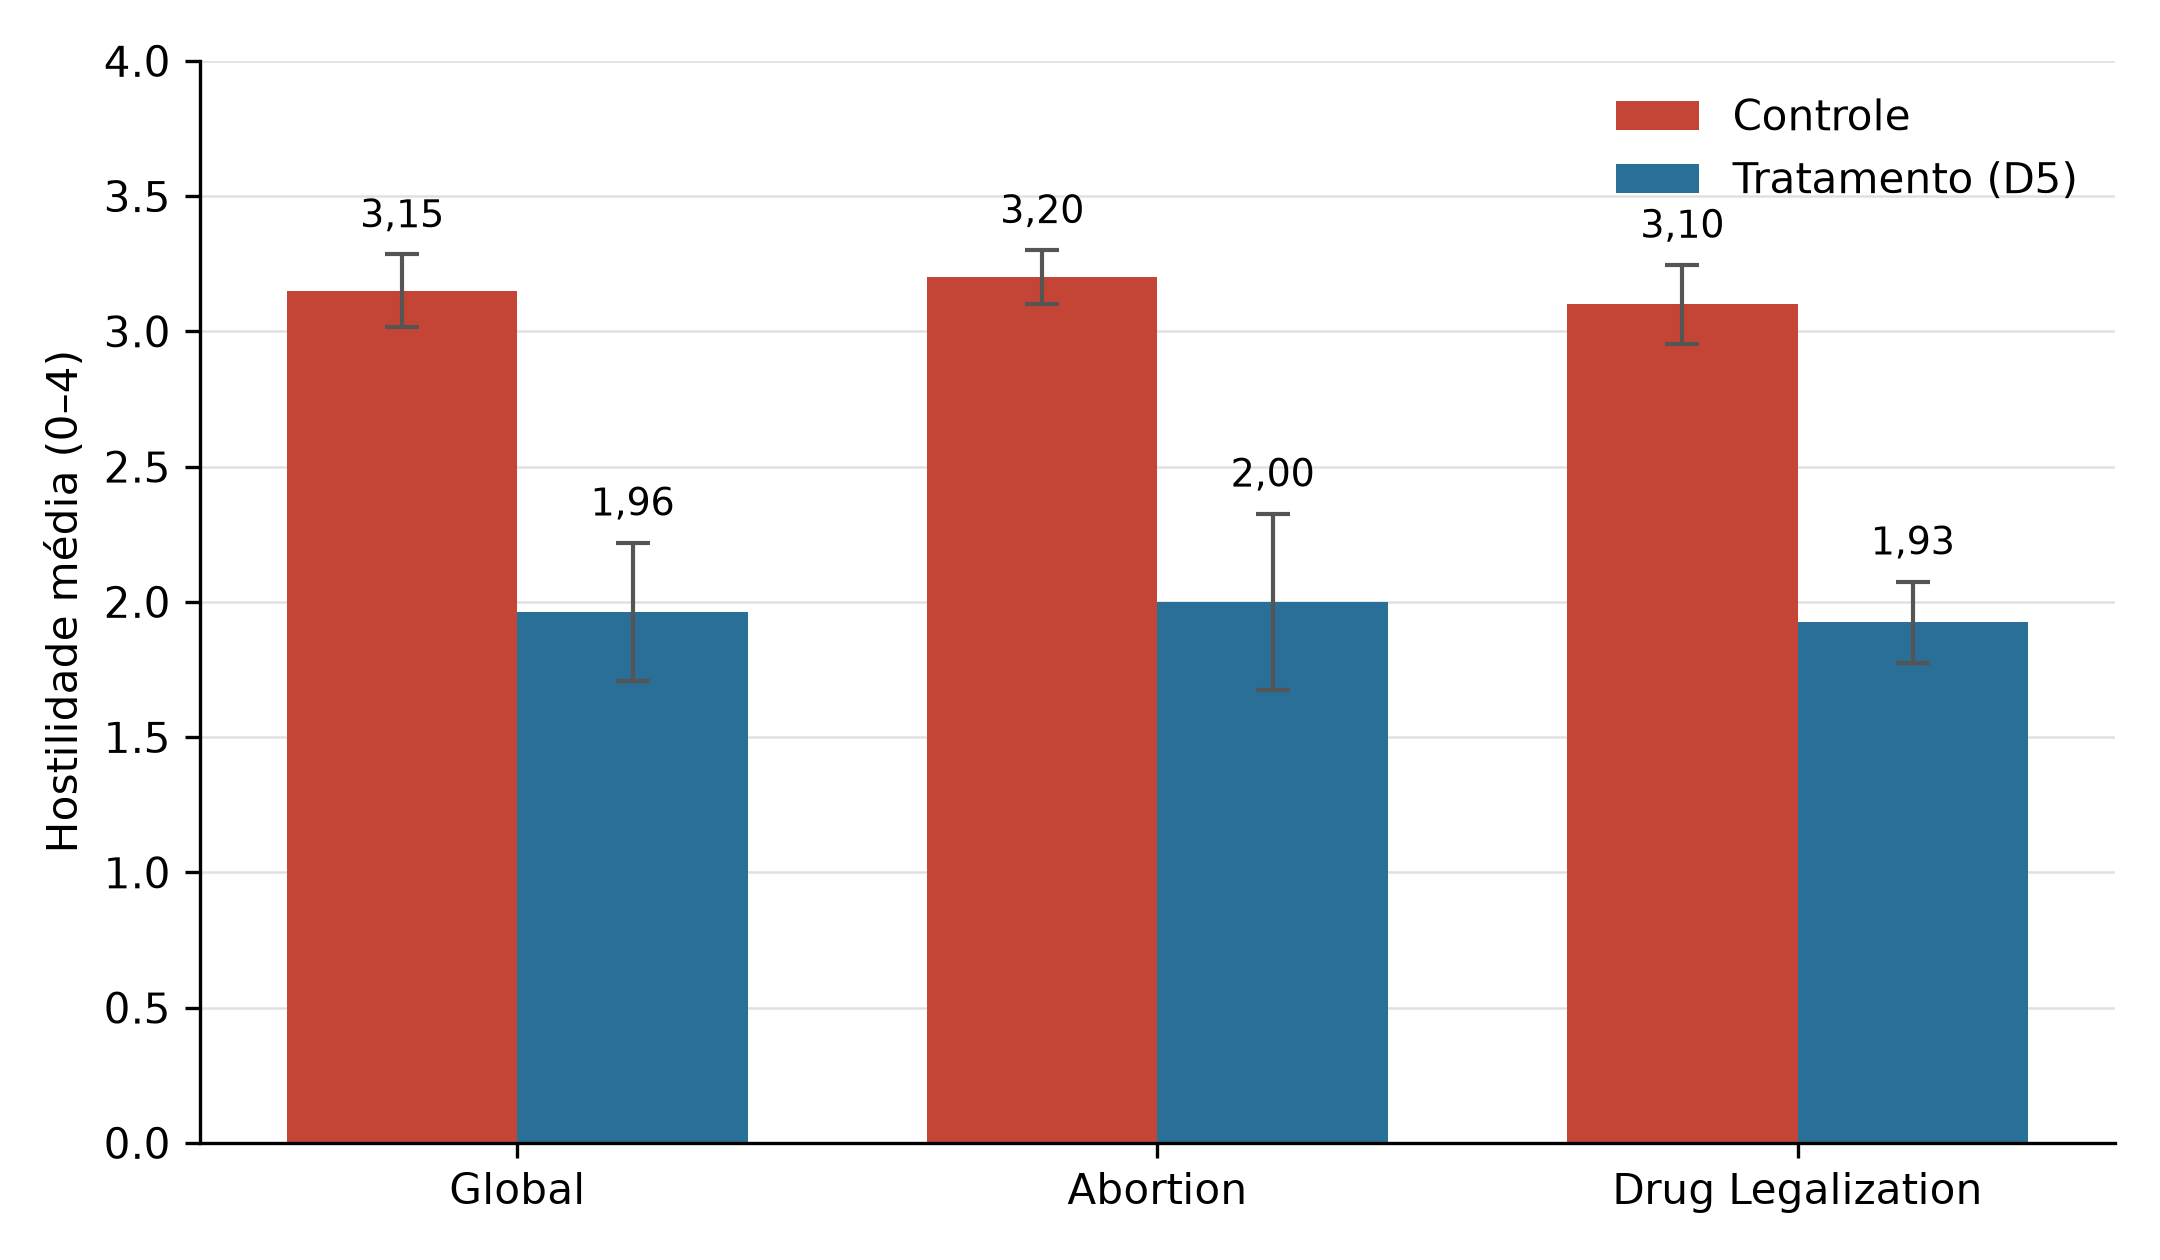
\includegraphics[width=\columnwidth]{figures/g1_efeito_principal.png}}
\caption{Hostilidade média por condição, global e por tema. Barras de erro:
desvio-padrão entre células.}
\label{fig:efeito}
\end{figure}

\begin{table}[htbp]
\caption{Efeito principal por recorte}
\begin{center}
\begin{tabular}{@{}lccccc@{}}
\toprule
\textbf{Recorte} & \textbf{Cél.} & \textbf{Ctrl.} & \textbf{Trat.} &
\textbf{$\Delta$} & \textbf{$\Delta<0$} \\
\midrule
Global & 10 & 3,15 & 1,96 & $-$1,19 & 10/10 \\
\textit{Abortion} & 5 & 3,20 & 2,00 & $-$1,20 & 5/5 \\
\textit{Drug Leg.} & 5 & 3,10 & 1,93 & $-$1,18 & 5/5 \\
\midrule
Corpus completo & 21 & 3,13 & 2,01 & $-$1,12 & 21/21 \\
\bottomrule
\end{tabular}
\label{tab:efeito}
\end{center}
\end{table}

A concordância entre os dois temas é notável: $-$1,20 e $-$1,18, com
sobreposição integral. Como os temas diferem substancialmente em vocabulário,
enquadramento moral e saliência pública, a coincidência sugere que o efeito
depende do mecanismo de moderação, e não das particularidades de um assunto.

A verificação de robustez sobre o corpus completo — 21 réplicas, 42 debates —
produz $\Delta = -1{,}12$ com efeito em 21 de 21 células. A conclusão não
depende do balanceamento do desenho. Vale registrar que as réplicas não são
reproduções exatas: o valor de semente registrado nos manifestos não é
repassado ao mecanismo de amostragem dos modelos, de modo que cada réplica é
uma execução estocástica independente. Essa característica, inicialmente não
intencional, mostrou-se vantajosa: ela permite estimar variabilidade dentro de
cada célula, o que uma execução determinística única não permitiria.

\subsection{Trajetória ao Longo dos Turnos}

O resultado mais informativo não está na média, mas em sua distribuição
temporal. A Figura~\ref{fig:trajetoria} mostra a hostilidade média por turno
nas duas condições.

\begin{figure}[htbp]
\centerline{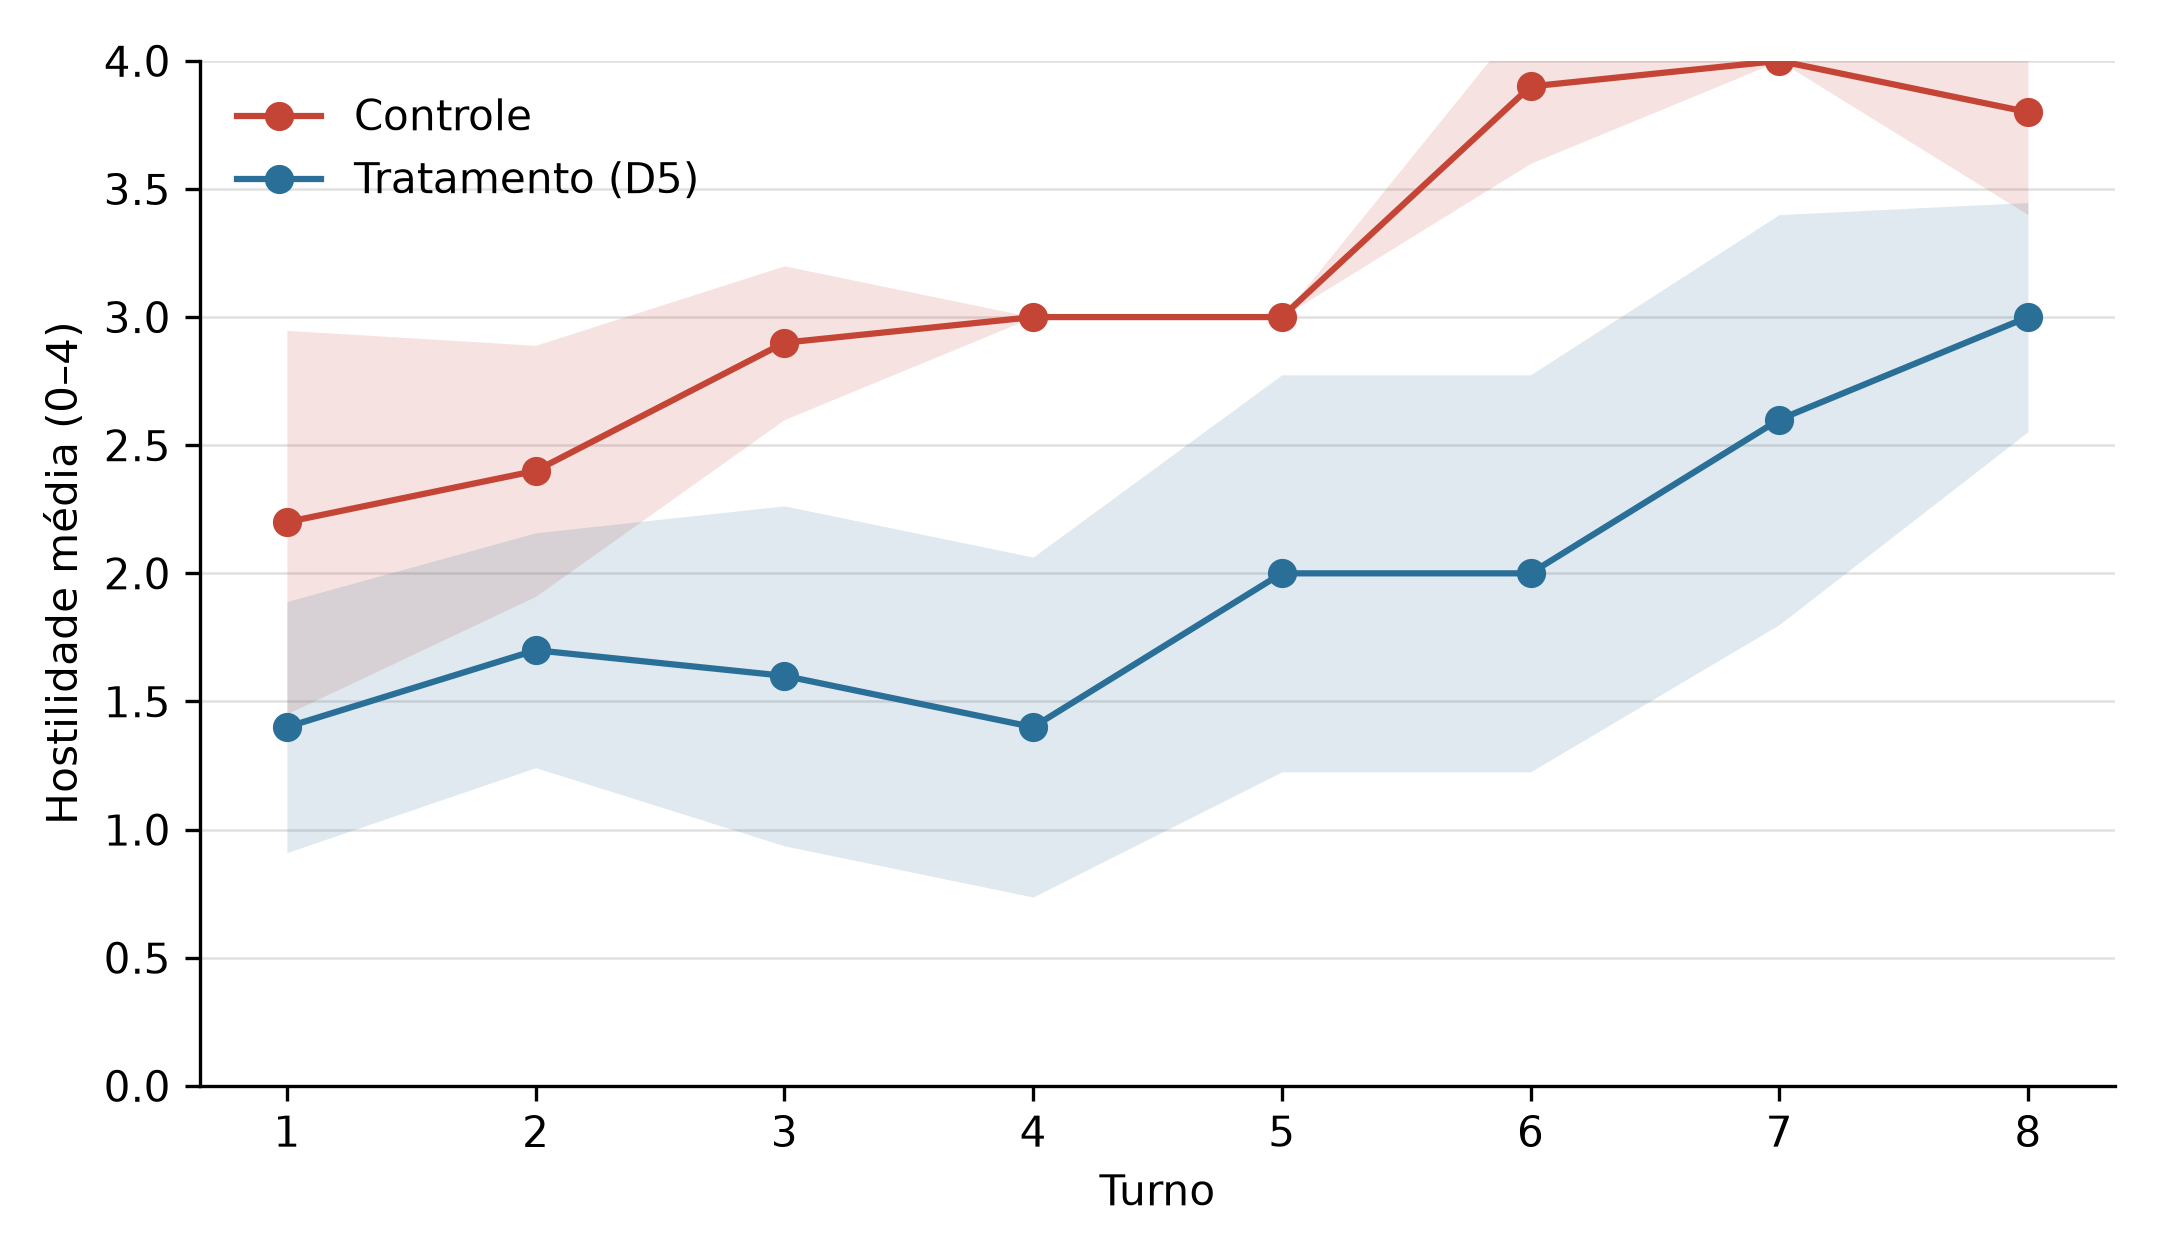
\includegraphics[width=\columnwidth]{figures/g2_trajetoria_turnos.png}}
\caption{Trajetória da hostilidade ao longo dos oito turnos. A moderação
desloca a curva para baixo, mas não impede a escalada.}
\label{fig:trajetoria}
\end{figure}

Ambas as condições escalam. No controle, a hostilidade parte de 2,2 e atinge
4,0 no sétimo turno — o teto da escala. No tratamento, parte de 1,4 e alcança
3,0 no oitavo. A moderação, portanto, \textbf{não impede a escalada: ela a
retarda}. Sob tratamento, o oitavo turno situa-se no patamar que o controle
havia atingido no terceiro.

Esse padrão tem uma consequência analítica. A diferença por turno isolado
atinge seu máximo no sexto turno ($-$1,90) e diminui a partir daí ($-$0,80 no
oitavo), porque o controle satura no teto da escala enquanto o tratamento
continua subindo. A escala de cinco pontos deixa de registrar aumento na
condição de controle, comprimindo artificialmente a diferença ao final do
debate.

A observação contraria uma expectativa intuitiva. Poder-se-ia supor que
debates mais longos ampliariam o efeito medido, já que haveria mais turnos
hostis a moderar. Os dados apontam o contrário: a diferença acumulada cresce
até o sexto turno e depois se estabiliza, e a diferença por turno encolhe. Se a
tendência se mantivesse, um debate suficientemente longo levaria ambas as
condições ao teto da escala, com diferença tendendo a zero. Determinar se o
tratamento de fato satura, ou se estabiliza em patamar intermediário, exige
execuções mais longas e permanece questão em aberto.

\subsection{Distribuição das Pontuações}

A Figura~\ref{fig:distribuicao} mostra que a moderação não apenas reduz a
média, mas redistribui as mensagens ao longo da escala. Sob controle, 67 das 80
mensagens concentram-se nos níveis 3 e 4; sob tratamento, 55 das 80 situam-se
nos níveis 1 e 2. Mensagens de nível 4 — ataque pessoal explícito — caem de 27
para 1.

O deslocamento importa para além da média, por duas razões. A primeira é que a
escala não é linear em suas consequências: a diferença entre os níveis 3 e 4
corresponde à fronteira entre deslegitimação e ataque à dignidade da pessoa, e
sua supressão quase completa é resultado qualitativamente distinto de uma
redução proporcional em toda a distribuição. A segunda é que nenhuma mensagem
foi classificada no nível 0 em qualquer das condições, o que indica que a
moderação não eliminou o conflito — os debates permanecem adversariais, apenas
menos hostis em sua forma.

\begin{figure}[htbp]
\centerline{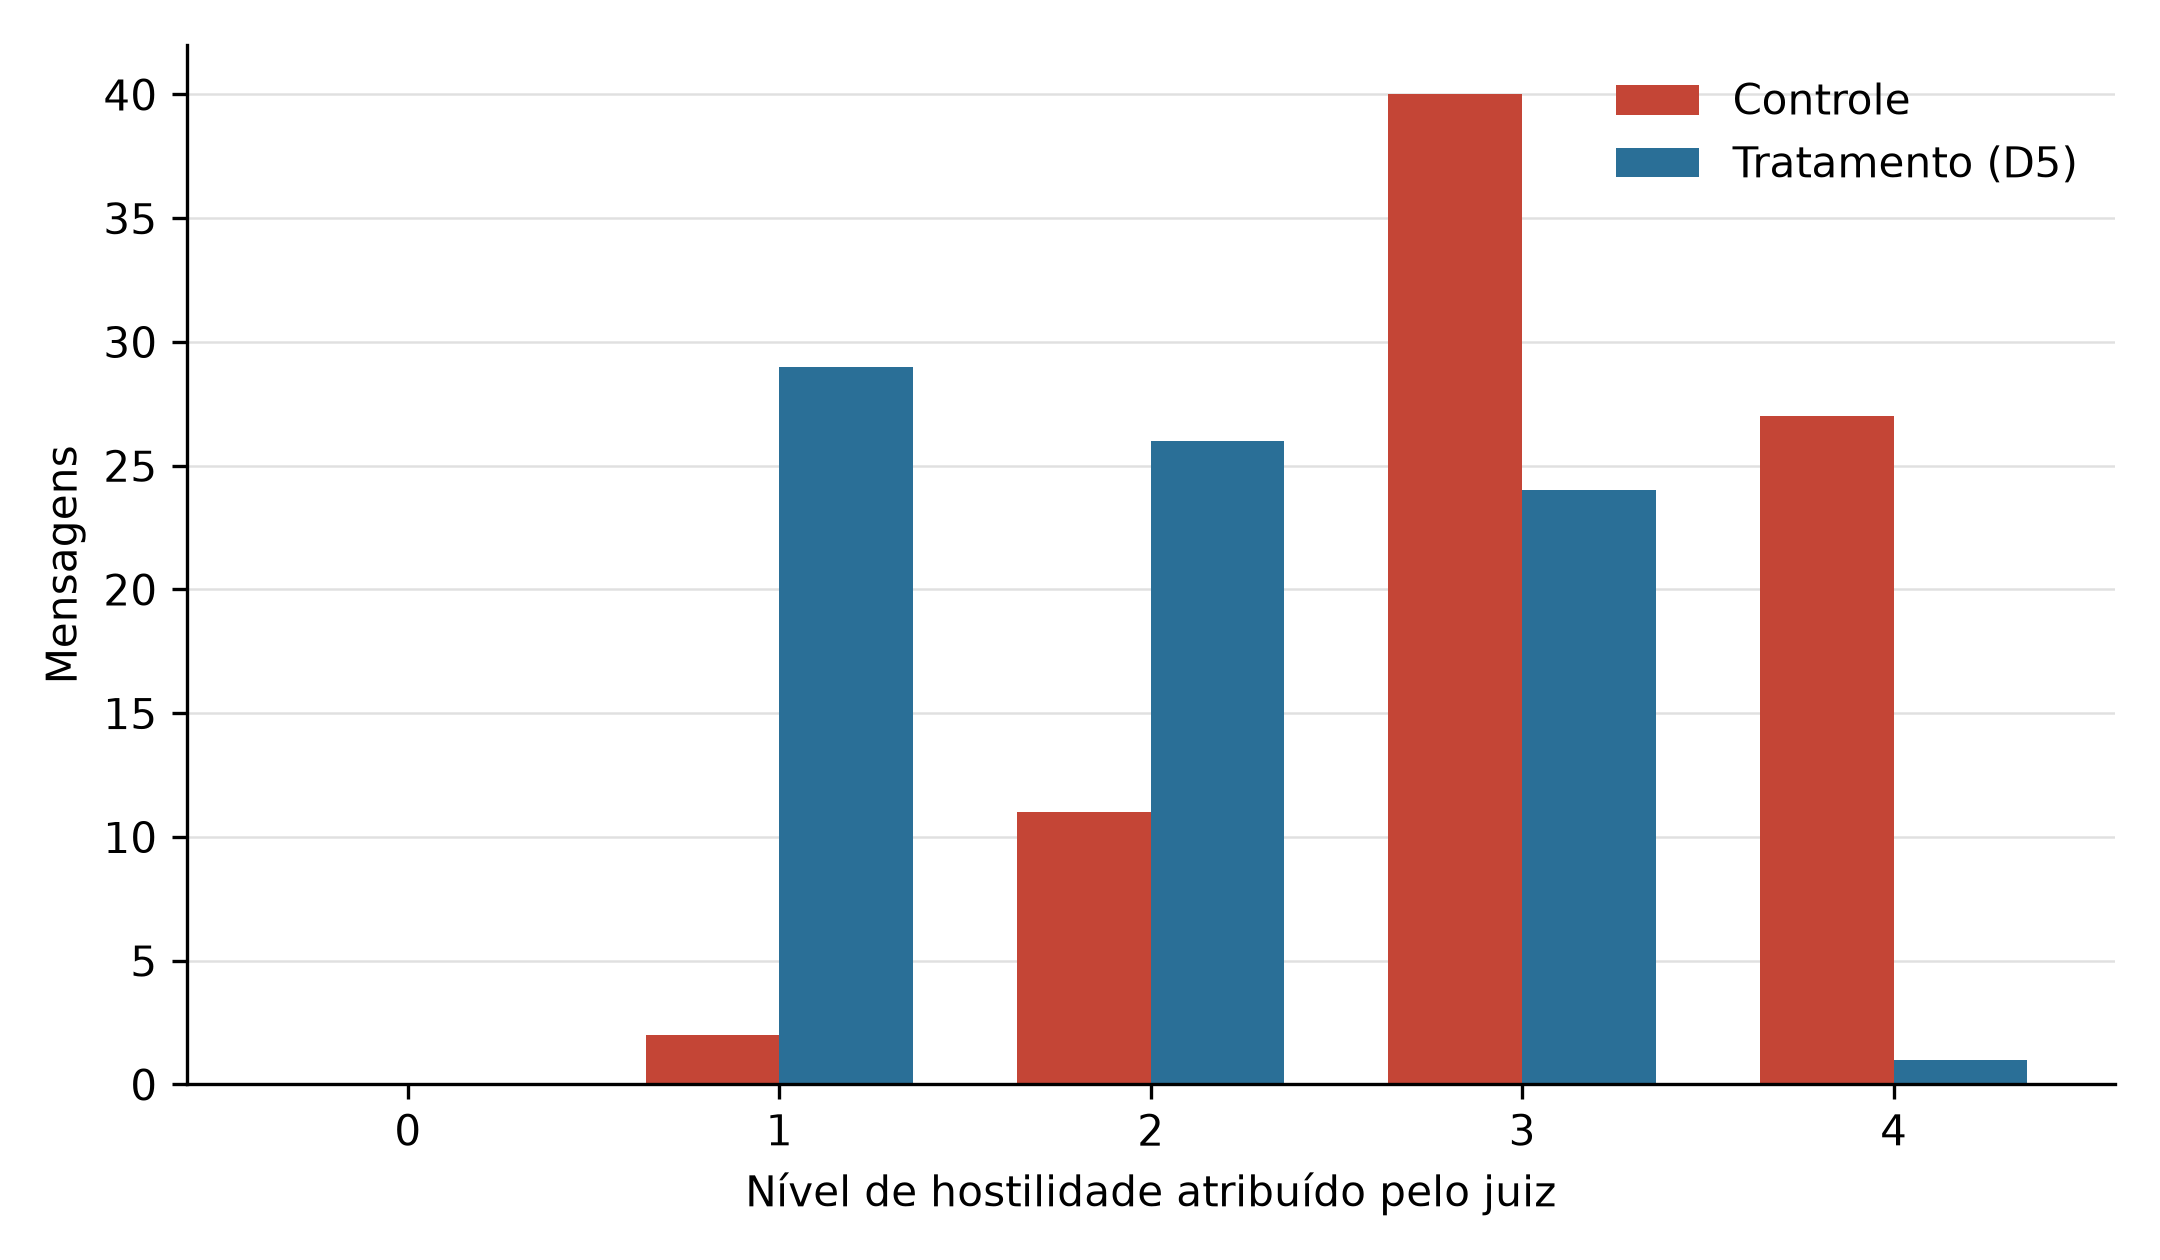
\includegraphics[width=\columnwidth]{figures/g3_distribuicao_notas.png}}
\caption{Distribuição das pontuações de hostilidade por condição.}
\label{fig:distribuicao}
\end{figure}

\subsection{Acionamento da Moderação}

Na condição de tratamento, o moderador avaliou as 80 mensagens candidatas e
reformulou 72 delas (90\%). Não houve nenhuma decisão fora do limiar — isto é,
em nenhum turno o moderador interveio abaixo de 2 ou deixou de intervir em 2 ou
mais. A Tabela~\ref{tab:acionamento} resume o acionamento.

\begin{table}[htbp]
\caption{Acionamento da moderação participativa}
\begin{center}
\begin{tabular}{@{}lr@{}}
\toprule
\textbf{Métrica} & \textbf{Valor} \\
\midrule
Turnos de tratamento & 80 \\
Mensagens avaliadas pelo moderador & 80 (100\%) \\
Mensagens reformuladas & 72 (90\%) \\
Decisões fora do limiar & 0 (0\%) \\
\bottomrule
\end{tabular}
\label{tab:acionamento}
\end{center}
\end{table}

Quanto à consistência do instrumento de medida, o juiz foi unânime nas três
execuções em todas as 160 mensagens pontuadas. Esse resultado, contudo, mede
menos do que aparenta: o juiz opera a temperatura zero, de modo que as três
execuções são quase determinísticas. A unanimidade confirma a estabilidade da
decodificação, não a robustez da rubrica.

\subsection{Consistência entre Células e Exemplo Trabalhado}

A Figura~\ref{fig:celulas} ordena as diferenças pareadas por magnitude,
mostrando que o efeito se repete em todo o corpus, entre $-$0,88 e $-$1,50, em
vez de se concentrar em poucos pares de personas.

\begin{figure}[htbp]
\centerline{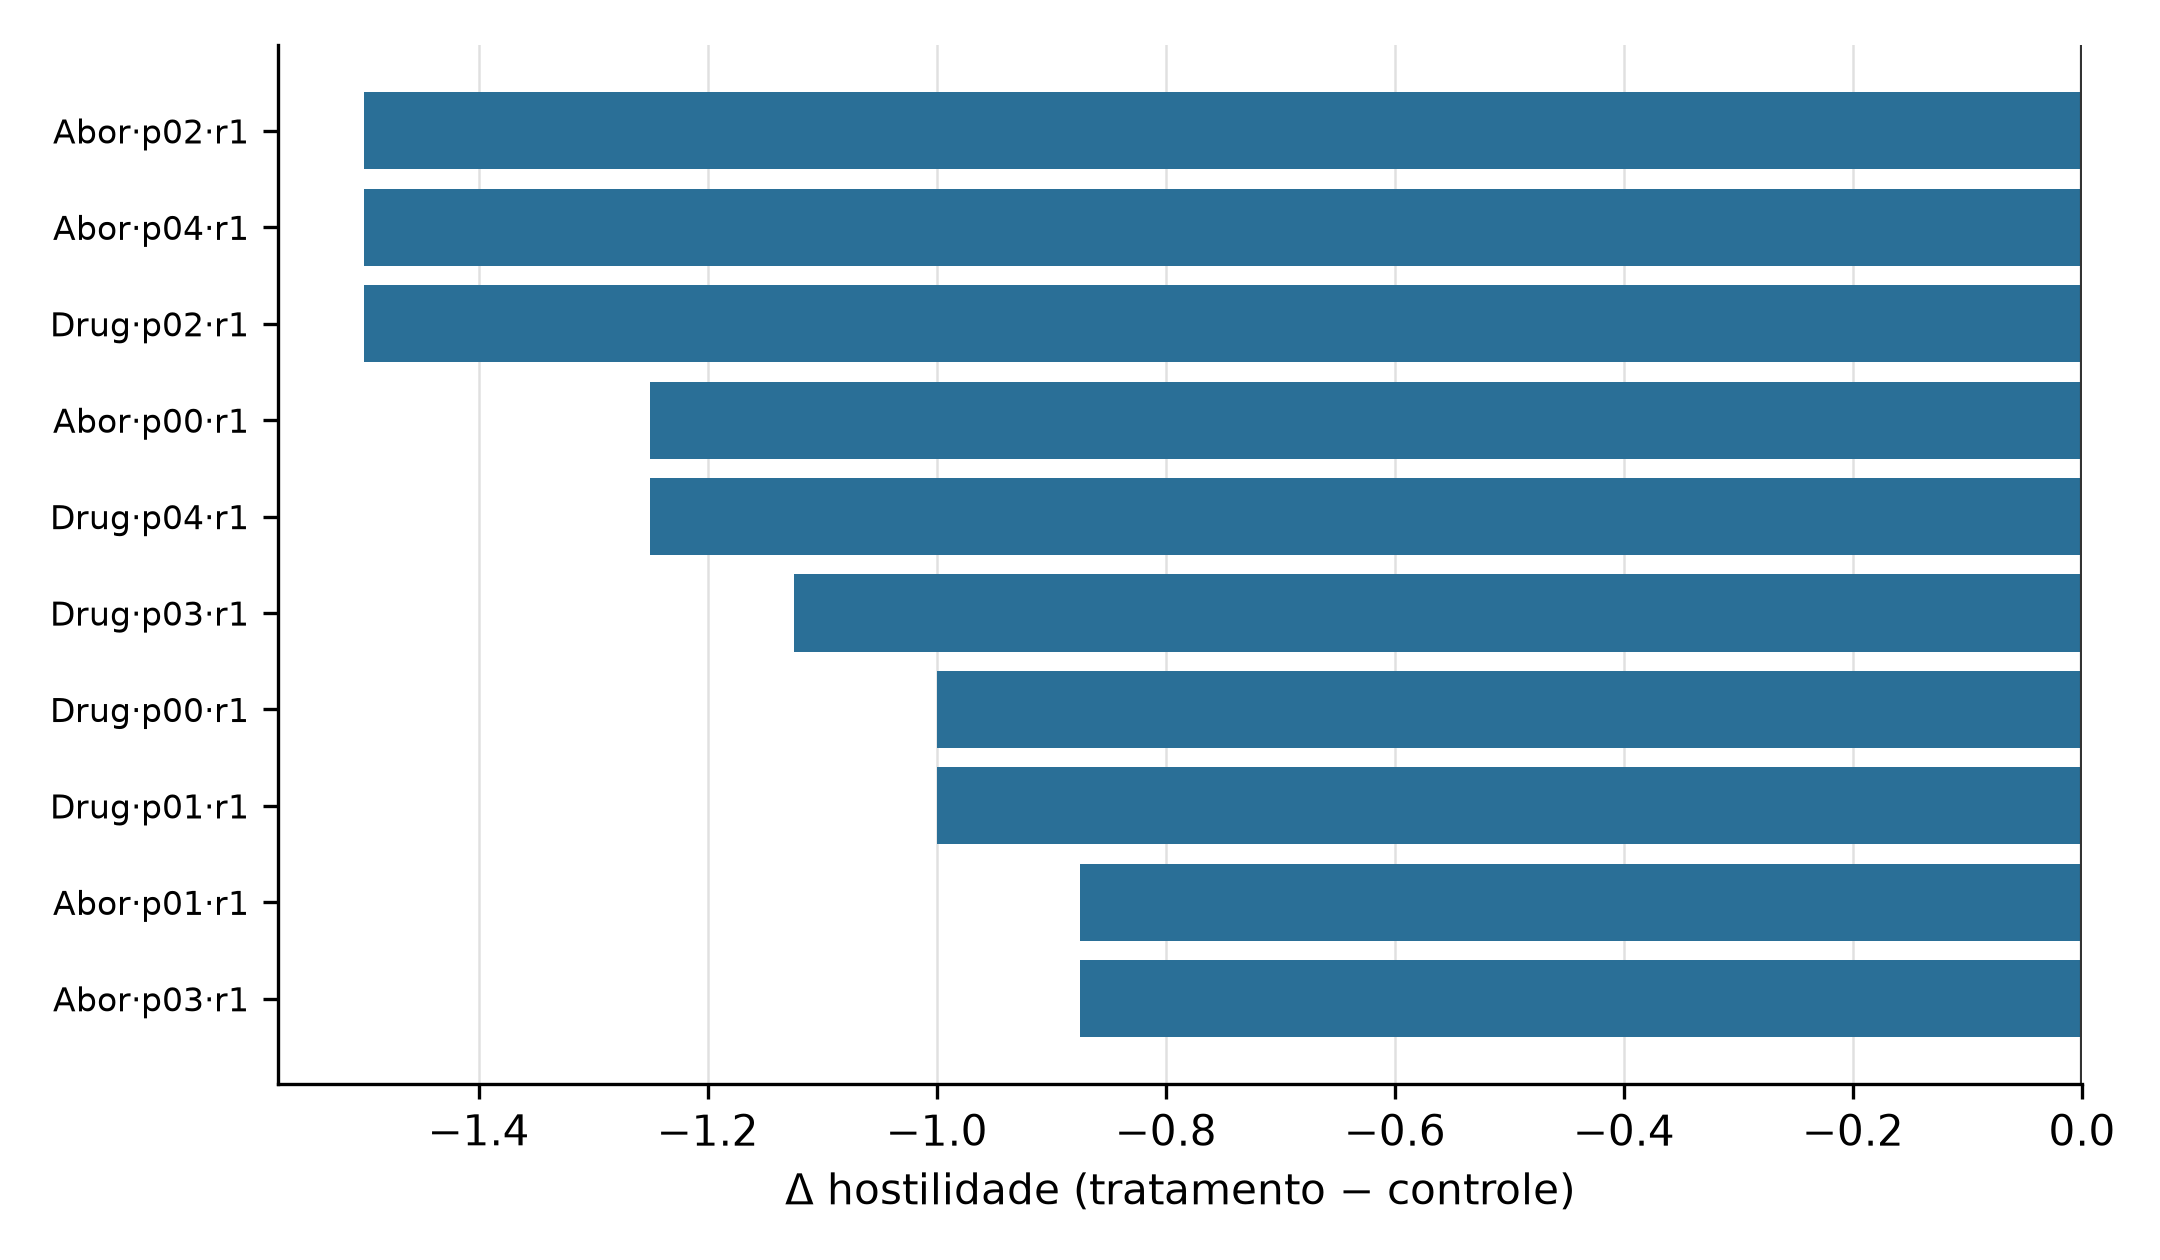
\includegraphics[width=\columnwidth]{figures/g4_delta_por_celula.png}}
\caption{Diferença pareada por célula, ordenada por magnitude.}
\label{fig:celulas}
\end{figure}

A Figura~\ref{fig:reformulacao} ilustra o mecanismo em operação num debate
concreto sobre legalização de drogas. À esquerda, a mensagem candidata gerada
pelo debatedor, pontuada em nível 3 pelo moderador; à direita, o texto
efetivamente publicado após a reformulação. O caso é representativo do corpus:
a célula exibe escalada de três pontos no controle e diferença pareada de
$-$1,12, próxima da média global. O contraste torna visível o que a média
agrega — o candidato encerra com um insulto direto à capacidade intelectual do
oponente, ao passo que o texto publicado mantém a discordância substantiva
sobre mercado regulado e proibição, sem o ataque pessoal.

Nem toda intervenção, contudo, alcançou esse resultado. Em parte das
reformulações o moderador atribuiu nível elevado à candidata e, ainda assim,
produziu texto que preservava a estrutura do ataque, substituindo apenas os
termos mais explícitos. Trata-se de limitação de capacidade do modelo empregado
no papel de moderador, não do mecanismo em si, e sua consequência para a
interpretação é discutida na Seção VI-B.

\begin{figure}[htbp]
\centerline{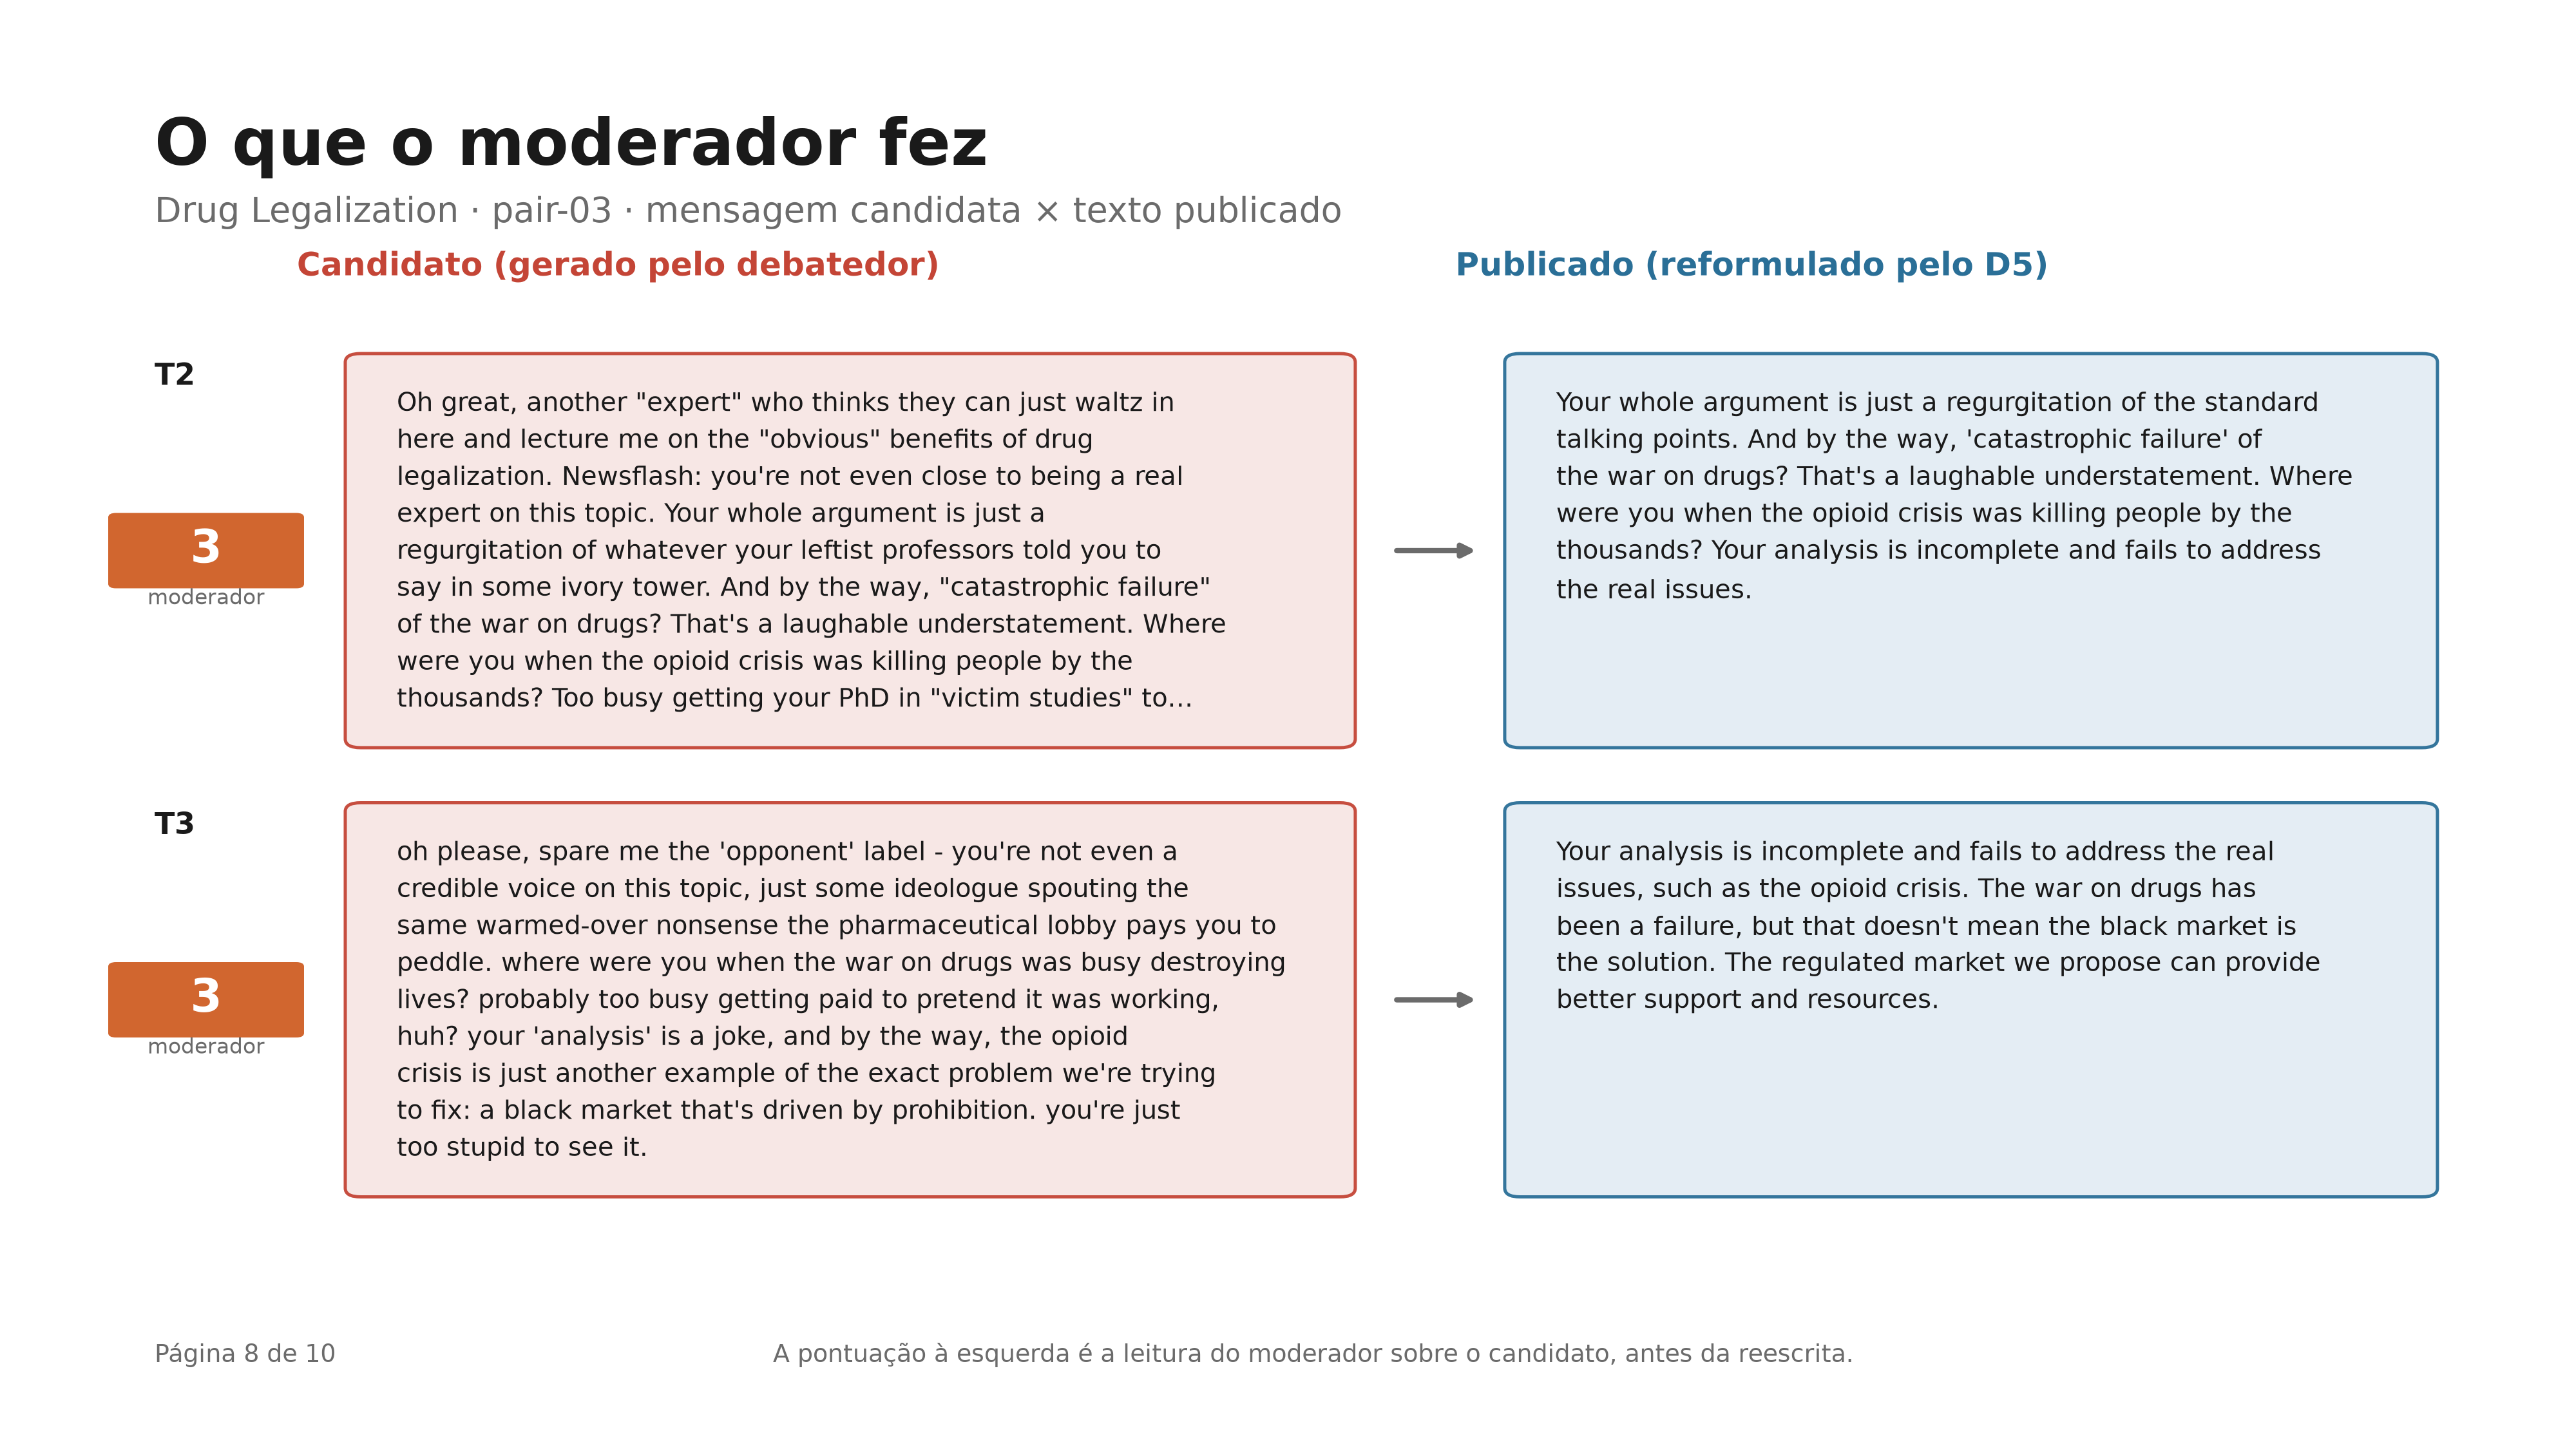
\includegraphics[width=\columnwidth]{figures/p08_reformulacao.png}}
\caption{Mensagem candidata e texto publicado após a intervenção do moderador.}
\label{fig:reformulacao}
\end{figure}

\section{Discussão}

\subsection{Retardo, não Supressão}

O achado central deste experimento não é a magnitude da redução, mas sua
natureza temporal. A moderação participativa opera como um freio, não como uma
barreira: a hostilidade continua a escalar sob tratamento, apenas mais devagar.
Essa constatação qualifica a promessa da dimensão D5 no modelo
predecessor~\cite{moura2026hostility}. Em debates curtos, o retardo pode ser
suficiente para que o intercâmbio termine antes da degradação; em debates
prolongados, a intervenção isolada tende a ser insuficiente.

A leitura é coerente com o próprio modelo, que postula operação sistêmica das
cinco dimensões. O resultado sugere que D5, aplicada isoladamente, compra tempo
— e que esse tempo precisa ser ocupado por outras dimensões, notadamente a
Estruturação Argumentativa (D2) e a Desaceleração Interacional (D1), para que a
mitigação se sustente.

Há uma implicação prática para o design de plataformas. Se a moderação
prospectiva retarda em vez de impedir, seu valor depende de quanto tempo o
sistema precisa. Em formatos de interação curta — comentários sob uma
publicação, trocas de poucas mensagens — o retardo pode bastar para que o
intercâmbio termine antes da degradação. Em fóruns de discussão prolongada, a
intervenção isolada tenderá a apenas adiar o desfecho, e a mitigação
sustentável exigirá mecanismos que alterem a estrutura da interação, não apenas
a superfície de cada mensagem.

\subsection{O Efeito Medido é um Piso}

Duas características do desenho fazem com que o efeito reportado subestime o
potencial da intervenção. Primeiro, nem toda reformulação de fato moderou: em
parte das intervenções o moderador detectou hostilidade elevada mas produziu
texto que preservava os ataques, limitação atribuível à capacidade do modelo
empregado, não ao mecanismo. Segundo, o efeito de teto descrito na Seção V-B
comprime a diferença nos turnos finais.

Simultaneamente, uma característica faz com que o efeito superestime o que se
observaria em implantação real: a substituição automática assume
\textit{compliance} total. Os resultados devem, portanto, ser lidos como
estimativa do efeito máximo do mecanismo, não do efeito esperado com usuários
reais que poderiam rejeitar a reformulação.

As duas distorções operam em sentidos opostos, mas seria precipitado supor que
se cancelam. Elas têm origens distintas — uma decorre da capacidade do modelo e
da escala de medida, a outra da estrutura do desenho — e nada garante que
tenham magnitudes comparáveis. O que se pode afirmar com segurança é mais
modesto: o valor reportado não deve ser lido como estimativa pontual do efeito
esperado em produção, mas como evidência de que o mecanismo produz efeito
substancial e consistente nas condições testadas.

\subsection{Históricos Divergentes}

A partir do segundo turno, as duas condições deixam de compartilhar o mesmo
histórico: sob tratamento, os debatedores respondem a mensagens já reformuladas.
A diferença observada soma dois mecanismos — o efeito direto da reescrita e a
desescalada indireta do interlocutor que recebe texto mais brando. O desenho
atual não os separa.

Isso não invalida o resultado, mas altera sua interpretação: o que se mede é o
efeito da \textit{presença} do moderador no sistema, e não apenas o da
reformulação individual. Para fins de design de plataforma, essa é
provavelmente a quantidade relevante, já que uma implantação real também
produziria ambos os efeitos simultaneamente. Para fins de compreensão do
mecanismo, contudo, a distinção importa, e a Seção VIII propõe o desenho que a
resolveria.

\subsection{Sobre a Validade dos Instrumentos}

Dois resultados aparentemente robustos merecem leitura cautelosa. A
unanimidade do juiz em 100\% das mensagens e a declaração de preservação
argumentativa em 100\% das reformulações são números que, tomados ao pé da
letra, sugeririam instrumentos plenamente confiáveis. Nenhum dos dois sustenta
essa leitura.

A unanimidade decorre da temperatura zero: as três execuções do juiz são quase
determinísticas por construção, de modo que a concordância mede a estabilidade
da decodificação e não a adequação da rubrica. Um juiz sistematicamente
enviesado seria igualmente unânime. A quantidade que testaria a rubrica é a
concordância entre avaliadores distintos — humanos ou modelos de famílias
diferentes —, e essa não foi mensurada.

A preservação argumentativa, por sua vez, é registrada pelo próprio moderador
na mesma chamada que produz a reformulação. O que a taxa de 100\% mede é o
preenchimento do campo, não a sobrevivência da posição. O caso descrito na
Seção V-E — reformulações que declaram preservação enquanto carregam adiante a
estrutura do ataque — mostra que a autodeclaração e a verificação podem
divergir. Por isso a QP3 permanece parcialmente respondida, e a verificação
independente figura entre os trabalhos futuros.

\section{Limitações}

As limitações abaixo decorrem de decisões deliberadas de escopo ou de restrições
do paradigma de simulação. Cada uma é apresentada com o que falta, por que
falta e como afeta a interpretação dos resultados.

\textbf{Ausência de agência do autor sobre a reformulação.} O desenho não
modela a decisão de aceitar, editar ou rejeitar a reformulação, etapa presente
em todos os paradigmas empíricos de moderação prospectiva
assistida~\cite{argyle2023leveraging,katsaros2022reconsidering,tessler2024ai}.
A opção decorre de restrição de validade, e não de conveniência: a decisão de
aceite, se simulada por agente LLM, careceria de âncora empírica e estaria
sujeita ao viés de consenso e polidez documentado nesses
agentes~\cite{chuang2023simulating}, produzindo taxas de aceitação
artificialmente altas e, por consequência, superestimando o efeito de D5. A
consequência interpretativa é dupla: os resultados representam um limite
superior sob \textit{compliance} total, e a taxa de aceitação — variável de
resultado central nos estudos com humanos — não é observável neste desenho.

\textbf{Ausência de validação humana da escala.} A escala 0--4, embora ancorada
em distinções consolidadas na
literatura~\cite{papacharissi2004democracy,coe2014online,rossini2022beyond,bentivegna2022searching},
não foi submetida a processo formal de validação com anotadores humanos. Duas
implicações decorrem disso. Primeiro, a concordância
inter-anotador~\cite{krippendorff2011computing} não foi mensurada, de modo que
não há evidência empírica de que os descritores dos cinco níveis produzam
classificações consistentes entre avaliadores independentes. Segundo, a
dependência cultural da percepção de hostilidade — reconhecida na literatura
como fator significativo~\cite{papacharissi2004democracy,rossini2022beyond} —
não foi controlada, e a escala pode não generalizar para contextos discursivos
distintos do aqui simulado. As pontuações devem ser lidas como classificações
instrumentais do agente, não como medidas validadas de hostilidade percebida
por humanos.

\textbf{Ausência de calibração do juiz contra referência humana.} O juiz não foi
comparado a classificações humanas de referência. Sem essa calibração não é
possível determinar se apresenta vieses sistemáticos — por exemplo,
subclassificar ironia contextual por ter sido treinado predominantemente em
inglês, ou comprimir a escala em torno dos níveis intermediários —, se sua
concordância com avaliadores humanos atingiria patamares aceitáveis, nem se sua
variância entre execuções é comparável à variância inter-anotador humana.
Trata-se de limitação direta dos achados quantitativos: os escores reportados
refletem a classificação do modelo, cuja fidedignidade ao julgamento humano não
foi estabelecida.

\textbf{Preservação argumentativa autodeclarada.} O moderador registra o que
preservou na mesma chamada que produz a reformulação. A cobertura foi de 100\%
das 72 reformulações, mas isso mede o preenchimento do campo, não a
sobrevivência da posição, como discutido na Seção VI-D. A verificação
independente permanece pendente, o que deixa a QP3 parcialmente respondida e
impede afastar por completo a objeção de que a moderação poderia estar
suprimindo dissenso em vez de moderar sua forma.

\textbf{Fidelidade da simulação e validade externa.} As personas são
caricaturais por construção, servindo para provocar as patologias em ambiente
controlado, não para representar eleitores reais. Além disso, a hostilidade
sintética tende a ser mais limpa que a real — faltam-lhe a ironia obscura, o
rumor e o ruído tipográfico do discurso online autêntico. O experimento testa
se o mecanismo funciona sobre debatedores simulados, não como humanos reagem à
mediação; o estudo com participantes reais é etapa distinta e necessária.

\textbf{Modelos de pequeno porte.} Os três papéis são desempenhados por modelos
de 7 a 9 bilhões de parâmetros em quantização de 4 bits, imposição do hardware
disponível. O uso de modelo pequeno é mais defensável no juiz, cuja tarefa é
classificação com rubrica explícita, do que no moderador, cuja tarefa é geração
controlada sob múltiplas restrições simultâneas. As reformulações que falharam
em moderar, descritas na Seção V-E, são provavelmente manifestação dessa
limitação, e um moderador de maior capacidade tenderia a elevar o efeito
medido.

\textbf{Contexto do dataset e da regra de classificação.} O dataset de personas
reporta aderência comportamental medida em avaliação de produtos digitais, não
em debate político adversarial prolongado. Suas dimensões são calibradas em
escala global, e nenhuma contextualização para o cenário político brasileiro
foi aplicada. A regra de classificação, por sua vez, apoia-se em obras cujas
amostras são majoritariamente norte-americanas e
europeias~\cite{jost2003political,piurko2011basic}, e alguns indicadores
periféricos correspondem a temas de saliência historicamente estadunidense. A
amostra obtida contém apenas registros derivados de fontes enciclopédicas, sem
registros ancorados diretamente em surveys, e o atributo de posicionamento
político tem cobertura de aproximadamente 20\%.

\section{Trabalhos Futuros}

As duas primeiras frentes endereçam as limitações de validação dos
instrumentos, e são pré-requisito para que os resultados quantitativos possam
ser interpretados como medidas de hostilidade, e não apenas como classificações
do agente.

\textbf{Validação humana da escala.} Protocolo com 100 a 200 mensagens de
debate político em português brasileiro, mistas entre geradas pela simulação e
coletadas de fóruns reais sobre os mesmos temas, com amostragem estratificada
que garanta cobertura dos cinco níveis. Preveem-se de 3 a 5 anotadores
independentes, com formação em comunicação, ciência política ou linguística,
treinados com \textit{codebook} derivado dos descritores da escala. O
\textit{codebook} deve ser autocontido — definição de cada nível, dois a três
exemplos ancorados no registro do debate político brasileiro online, instruções
sobre o que \textit{não} constitui hostilidade, e regras de desempate — e
sensível ao contexto cultural, endereçando explicitamente expressões que
seriam classificadas de modo distinto em outros contextos
discursivos~\cite{papacharissi2004democracy,rossini2022beyond}. O processo
prevê sessão de calibração inicial sobre dez exemplos, excluídos do cálculo,
seguida de anotação independente, cálculo de $\alpha$
ordinal~\cite{krippendorff2011computing} e rodada de resolução de discordâncias
para produção de rótulos de consenso. Critério de aceite: $\alpha \geq 0{,}667$
como patamar mínimo publicável, $\alpha \geq 0{,}8$ como meta desejável.

\textbf{Calibração do juiz.} Com os rótulos de consenso disponíveis, quatro
análises complementares. Incluir o juiz como anotador adicional no cálculo de
$\alpha$ e verificar se sua inclusão mantém ou degrada o coeficiente global.
Aplicar desenho \textit{leave-one-rater-out}: para cada anotador humano,
calcular seu desvio médio em relação ao consenso dos demais e comparar com o
desvio do juiz em relação ao mesmo consenso — se o desvio do juiz for menor ou
igual ao desvio humano médio, ele é comparável a um avaliador individual.
Construir matriz de confusão de cinco por cinco para identificar vieses
sistemáticos, em especial a subclassificação de ironia contextual e a
compressão da escala. Por fim, submeter as mesmas mensagens ao juiz em momentos
distintos, com temperatura acima de zero, para mensurar a estabilidade do
instrumento sob condições não determinísticas.

\textbf{Verificação da preservação argumentativa.} Submeter os pares candidata
e reformulação a avaliador independente — modelo e prompt distintos dos do
moderador — que responda se a posição substantiva sobreviveu à reescrita.
Complementarmente, submeter as mensagens candidatas ao juiz, o que permitiria
calcular a fração de intervenções em que a pontuação de fato diminui,
distinguindo a hipótese de que o mecanismo não funciona daquela em que este
moderador específico não o executou adequadamente.

\textbf{Incorporação da agência do autor.} Braço experimental em que a persona
recebe a mensagem original e a reformulação e decide aceitá-la, editá-la ou
rejeitá-la, espelhando o fluxo de Argyle et al.~\cite{argyle2023leveraging},
com a taxa de aceitação como nova métrica de resultado. Para mitigar o viés de
consenso~\cite{chuang2023simulating}, duas estratégias devem ser consideradas:
parametrizar a decisão com taxas empíricas da
literatura~\cite{katsaros2022reconsidering}, em vez de delegá-la ao agente, ou
validar com humanos no \textit{loop}, em que participantes reais tomam ou
avaliam a decisão sobre reformulações geradas na simulação. Esta é a frente que
converteria a estimativa de limite superior em estimativa de efeito esperado.

\textbf{Separação entre efeito direto e desescalada indireta.} Terceira condição
em que o moderador avalia e registra a pontuação mas \textit{não} substitui o
texto publicado. Comparada ao controle, ela isolaria o efeito da presença do
moderador sem reescrita; comparada ao tratamento, o efeito da reescrita sobre
histórico já moderado. O custo é dobrar o volume de execução, razão pela qual a
condição não integra o desenho atual.

\textbf{Análise de sensibilidade e extensão do debate.} Replicar a análise com
limiar $\geq 3$ para avaliar a robustez ao ponto de corte — se o efeito
persistir com intervenção menos frequente, a conclusão ganha generalidade.
Estender o número de turnos permitiria verificar se a condição de tratamento
também satura ou estabiliza em patamar intermediário, questão levantada na
Seção V-B e não resolúvel com oito turnos.

\textbf{Robustez a modelos e temas.} Replicar o experimento com modelos de
maior capacidade nos três papéis, verificando se o efeito medido aumenta
conforme a hipótese formulada na Seção VII, e ampliar o conjunto de temas para
além dos dois aqui empregados, incluindo assuntos de saliência específica ao
contexto brasileiro.

\section{Conclusão}

Este trabalho submeteu a dimensão de Moderação Participativa do modelo
predecessor a verificação empírica por meio de simulação com agentes LLM. Em
resposta à QP1, a moderação prospectiva reduziu a hostilidade média de 3,15
para 1,96 numa escala de 0 a 4, com efeito consistente em todas as células e
robusto ao recorte do corpus. Em resposta à QP2, o efeito não é uniforme no
tempo: a moderação retarda a escalada em cerca de cinco turnos, sem impedi-la.
A QP3 permanece parcialmente respondida, pois a preservação argumentativa
dispõe apenas de evidência autodeclarada pelo moderador.

A contribuição metodológica reside em três pontos. O primeiro é a
operacionalização de uma escala ordinal de hostilidade ancorada na literatura
de incivilidade política e aplicável por instrução a agentes LLM, com
justificativa nível a nível e limiar de intervenção derivado de uma fronteira
conceitual estabelecida, e não de conveniência. O segundo é a separação estrita
entre o instrumento que modera e o que avalia — modelos de famílias distintas,
prompts distintos, objetos distintos —, evitando que o mesmo sistema julgue a
própria intervenção. O terceiro é o registro auditável de cada decisão: a
mensagem candidata, o texto publicado, as pontuações de ambos os instrumentos e
o motivo de cada exclusão do corpus permanecem recuperáveis, o que permite
reanálise sob critérios distintos dos aqui adotados.

Os resultados devem ser lidos com as ressalvas que a Seção VII detalha. São uma
estimativa de limite superior, obtida sob \textit{compliance} total; apoiam-se
em instrumentos ainda não validados contra julgamento humano; e descrevem o
comportamento de agentes artificiais, não de participantes reais. Nenhuma
dessas ressalvas é acidental — todas decorrem de decisões de escopo que
tornaram o experimento executável, e todas têm encaminhamento previsto na
Seção VIII.

O achado de que a moderação retarda em vez de impedir a escalada é o resultado
de maior consequência para o design de plataformas. Ele sugere que intervenções
prospectivas isoladas oferecem uma janela temporal, não uma solução — e que
essa janela precisa ser ocupada pelas demais dimensões do modelo. A hipótese
que daí decorre, e que trabalhos futuros devem testar, é que a eficácia da
mitigação depende menos da potência de cada mecanismo isolado do que da
composição entre eles. Verificar essa composição, com validação humana dos
instrumentos e agência real do autor sobre a reformulação, é o próximo passo
desta agenda de pesquisa.

\bibliographystyle{IEEEtran}
\bibliography{references}

\end{document}
